\documentclass[12pt,letterpaper]{article}

%Packages
% \usepackage{textcomp}
% \usepackage{latexsym}
% \usepackage{url}
% \usepackage{amssymb}
% \usepackage{amsmath}
% \usepackage{mathtools}
% \usepackage{bm}
% \usepackage{array}
% \usepackage[version=3]{mhchem}
% \usepackage{ifthen}
% \usepackage{amsthm}
% \usepackage{amstext}
% \usepackage{enumerate}
% \usepackage{dcolumn}

\usepackage{epsfig}
\usepackage{graphicx}
\usepackage{caption}
\usepackage{hyperref}
\usepackage{lineno}
\usepackage{pdflscape}
\usepackage{mathtools}
\usepackage[osf]{mathpazo}
\usepackage{fullpage}
\usepackage{float}
\usepackage{xr} %linking to supplementaries
\usepackage{xcolor}
\externaldocument{supplementaries}

\pagenumbering{arabic}


%---------------------------------------------
%
%       START
%
%---------------------------------------------

\begin{document}
\noindent \today
\bigskip

\noindent Dear editor,
\bigskip

We are grateful for the detailed and useful comments from all four reviewers. We have taken all their suggestions on board, integrated changes associated with the suggestion into the manuscript and responded to them in detail below. For clarity we have displayed \textcolor{blue}{the reviewers’ comments in blue} and our own responses in black.

We have revised  the manuscript taking advantage of the extra space and number of figures allowed for Science Advances. Briefly, the major changes are:

\begin{itemize}
    \item We now clearly distinguish the two types of elaboration and innovation: $elaboration_{species}$ and $innovation_{species}$ that focuses on the macro-evolutionary scale and $elaboration_{clades}$ and $innovation_{clades}$ that focuses on the mega-evolutionary scale;
    \item For the analyses on elaboration and innovation at the macro scale ($elaboration_{species}$ and $innovation_{species}$), we now only focus on the projection of species onto their order’s major axes;
    \item We added two new figures and a table in the main text: the cheat sheet figure (previously in the supplementaries, now in the introduction), the correlation figure and a table from the new PGLS results; 
    \item We have added several new analyses to the supplementary materials including: correlations between elaboration/innovation, elaboration and innovation through time and random skewers analysis;
    \item We have linked our metrics definitions to previous work in the supplementary materials;
    \item We have made the vocabulary more consistent throughout the manuscript;
    \item We fully rewrote the introduction and most of the results/discussion section.
\end{itemize}

We fully describe each change below.
\bigskip
Best regards,
\bigskip
Thomas Guillerme, on behalf of all co-authors.

\section*{\textcolor{blue}{Reviewer 1}}

\textcolor{blue}{This study is an important contribution to the field of phenotypic macroevolution, and I strongly recommend its publication. The conceptualisation is very interesting, and I am aware that it represents the culmination of many years of research by the group/s involved, whose contributions I have seen several times along the years in several conferences. The authors devise a smart new method to evaluate the contributions of elaboration (i.e., evolutionary change along the major axis of variation of a clade) against innovation (i.e., evolutionary change away from this major axis).}

\textcolor{blue}{However, I have one major problem with the interpretation of the results. I will use an example to illustrate my point:}

\textcolor{blue}{Lines 108-110 go: ‘For example, compared to the global phylogenetic major axis of phenotypic variation, the Trochilidae (hummingbirds) in the order Apodiformes, have long narrow beaks and display high levels of elaboration and low innovation’.}

\textcolor{blue}{One could argue that the beak shape of hummingbirds represents one of the most exceptional cases of niche expansion and beak shape innovation in birds (Cooney, Bright et al., 2017, Nature). We know from the fossil record that hummingbirds likely evolved from broad-billed ancestors (i.e., stem trochilid Parargornis) so in reality, this comparison might not faithfully represent the actual evolutionary process undergone by crown group hummingbirds (high innovation as it departs from the main axis of evolutionary variation within strisoreans). Therefore, I am not sure I see what species values of ‘innovation’ and ‘elaboration’ in this context (i.e., compared to the global axis of whole-Neornithes variation) are telling us about the actual underlying innovation and elaboration as real evolutionary forces.}

\textcolor{blue}{I think the appropriate comparison for species values of innovation and elaboration might be with the main axes of variation of the immediately superior phylogenetic scale (order level in this case). Comparisons of species level values derived from the main axis of variation at the level of whole Neornithes might reflect global constraints in beak shape. For instance, coming back to the hummingbirds, there is some evidence that the divergence in cranial shape between hummingbirds and the remaining strisoreans might be related with a reversal to an ontogenetic trajectory that is pervasive among non- strisorean birds (Navalon et al., 2021, Proc. B). The similarities in beak shape between hummingbird species and the main axis of beak shape variation (long and slender to short and stout) in this study might reflect general constraints in beak shape variation rather than anything else. I think therefore conflating species level data from the whole-Neornithes axis with species level data from the order or parvorder axes might be confounding two kinds of data, different in nature, although, admittedly, it is intriguing that the same pattern (elaboration higher than innovation) holds at all the different phylogenetic levels.}

\textcolor{blue}{I suggest therefore keeping only the species level values as compared with the main axis of variation at the order/parvorder level as indicating ‘true’ innovation and elaboration. The comparisons of the main axis between different clades, in my opinion, indicate deep divergences in the main axes of beak shape variation. So I suggest keeping those too. Then either ditching the comparisons of species level dispersion values with whole- Neornithes or reinterpreting them.}

\textcolor{blue}{As a result, I am not entirely convinced with the authors conclusion that accumulated gradual elaboration creates deep divergences among main axes of variation in clades. I might be wrong, but my reading of the presented data is that:
\begin{enumerate}
\item Deep divergences among clades create different patterns of beak shape variation in different orders.
\item Species level beak shape variation within clades is characterised by more elaboration than innovation – evolution along lines of least resistance.
\item Species level variation as compared with the main axis of beak shape variation in whole Neornithes indicates that beak shapes are affected by whole-clade constraints – possibly of developmental nature. Calling this innovation and elaboration and equating it to the concepts in bullet point 2 is confusing in my opinion because it is several levels detached from the actual evolutionary process creating ‘elaboration’ or ‘innovation’.
\end{enumerate}
I reckon my interpretation is aligned with what earlier work by the authors (Cooney, Bright et al., 2017 and more by other authors!) suggest and adds to the discussion by showing the very interesting result that evolutionary variation in beak shape is largely constrained at several levels. But I don’t think it really contributes to ascertaining why deep divergences among clades occur unless further analyses can be carried out.}

We are grateful to the reviewer for pointing out this concern so clearly. We have now clarified what we mean by innovation and elaboration throughout the manuscript. We now consider the following:
\begin{itemize}
    \item Elaboration and innovation at the macroevolutionary scale for each species ($elaboration_{species}$ and $innovation_{species}$) as the projection/rejection of individual species on their order’s major axis of trait variance-covariance. We have moved the projections/rejection of species onto higher taxonomic levels (super-orders and the whole phylogeny) into the supplementary materials.
    \item Elaboration and innovation at the megaevolutionary scale (sensu Simpson 1944, 1953) $elaboration_{clade}$ and $innovation_{clade}$) as the projection/rejection of entire clades (orders or super-orders) onto their higher clades (super-order or the whole phylogeny).
\end{itemize}
We have reframed the whole manuscript and analyses with this in mind and have completely rewritten the introduction. Note that our previous version of the manuscript was a submission to Science and was directly transferred to Science Advances. We have now fully taken advantage of the extra space available which hopefully increases the clarity of the manuscript. This re-framing should remove the issues raised by the reviewer regarding the interpretations of our results.

We now also directly refer to the example suggested by this reviewers on lines 73-77:%@L_strisores_example:

\noindent\textit{For example, a major shift in beak shape arises in the early divergence of Strisores separating hummingbirds (Trochilidae) from swifts (Apodidae), perhaps marking changes in ontogenetic trajectories \cite{navalon2021} as hummingbirds diverged from broad billed ancestors (e.g. the Eocene stem Trochilidae fossils \textit{Parargornis messelensis} and \textit{Eocypselus rowei} \cite{mayr2003new, ksepka2013fossil}).} %@L_strisores_example


\textbf{\textcolor{blue}{More detailed comments:}}

\textcolor{blue}{I think Figure S5 – or a simplified version of it - should be Figure 1 in the main text to guide the readers through the methods and the theoretical framework used in the study. This will be beneficial too for the published paper to be noticed by the community – which I think it might be desirable because it is a very interesting contribution.}

Thanks for the suggestion. We have now reworked Figure S5 and use it as a “cheat sheet” in the introduction to guide the reader through the results of the original figures 1 and 2 (now figures 2 and 4).

\begin{figure}[!htbp]
\centering
   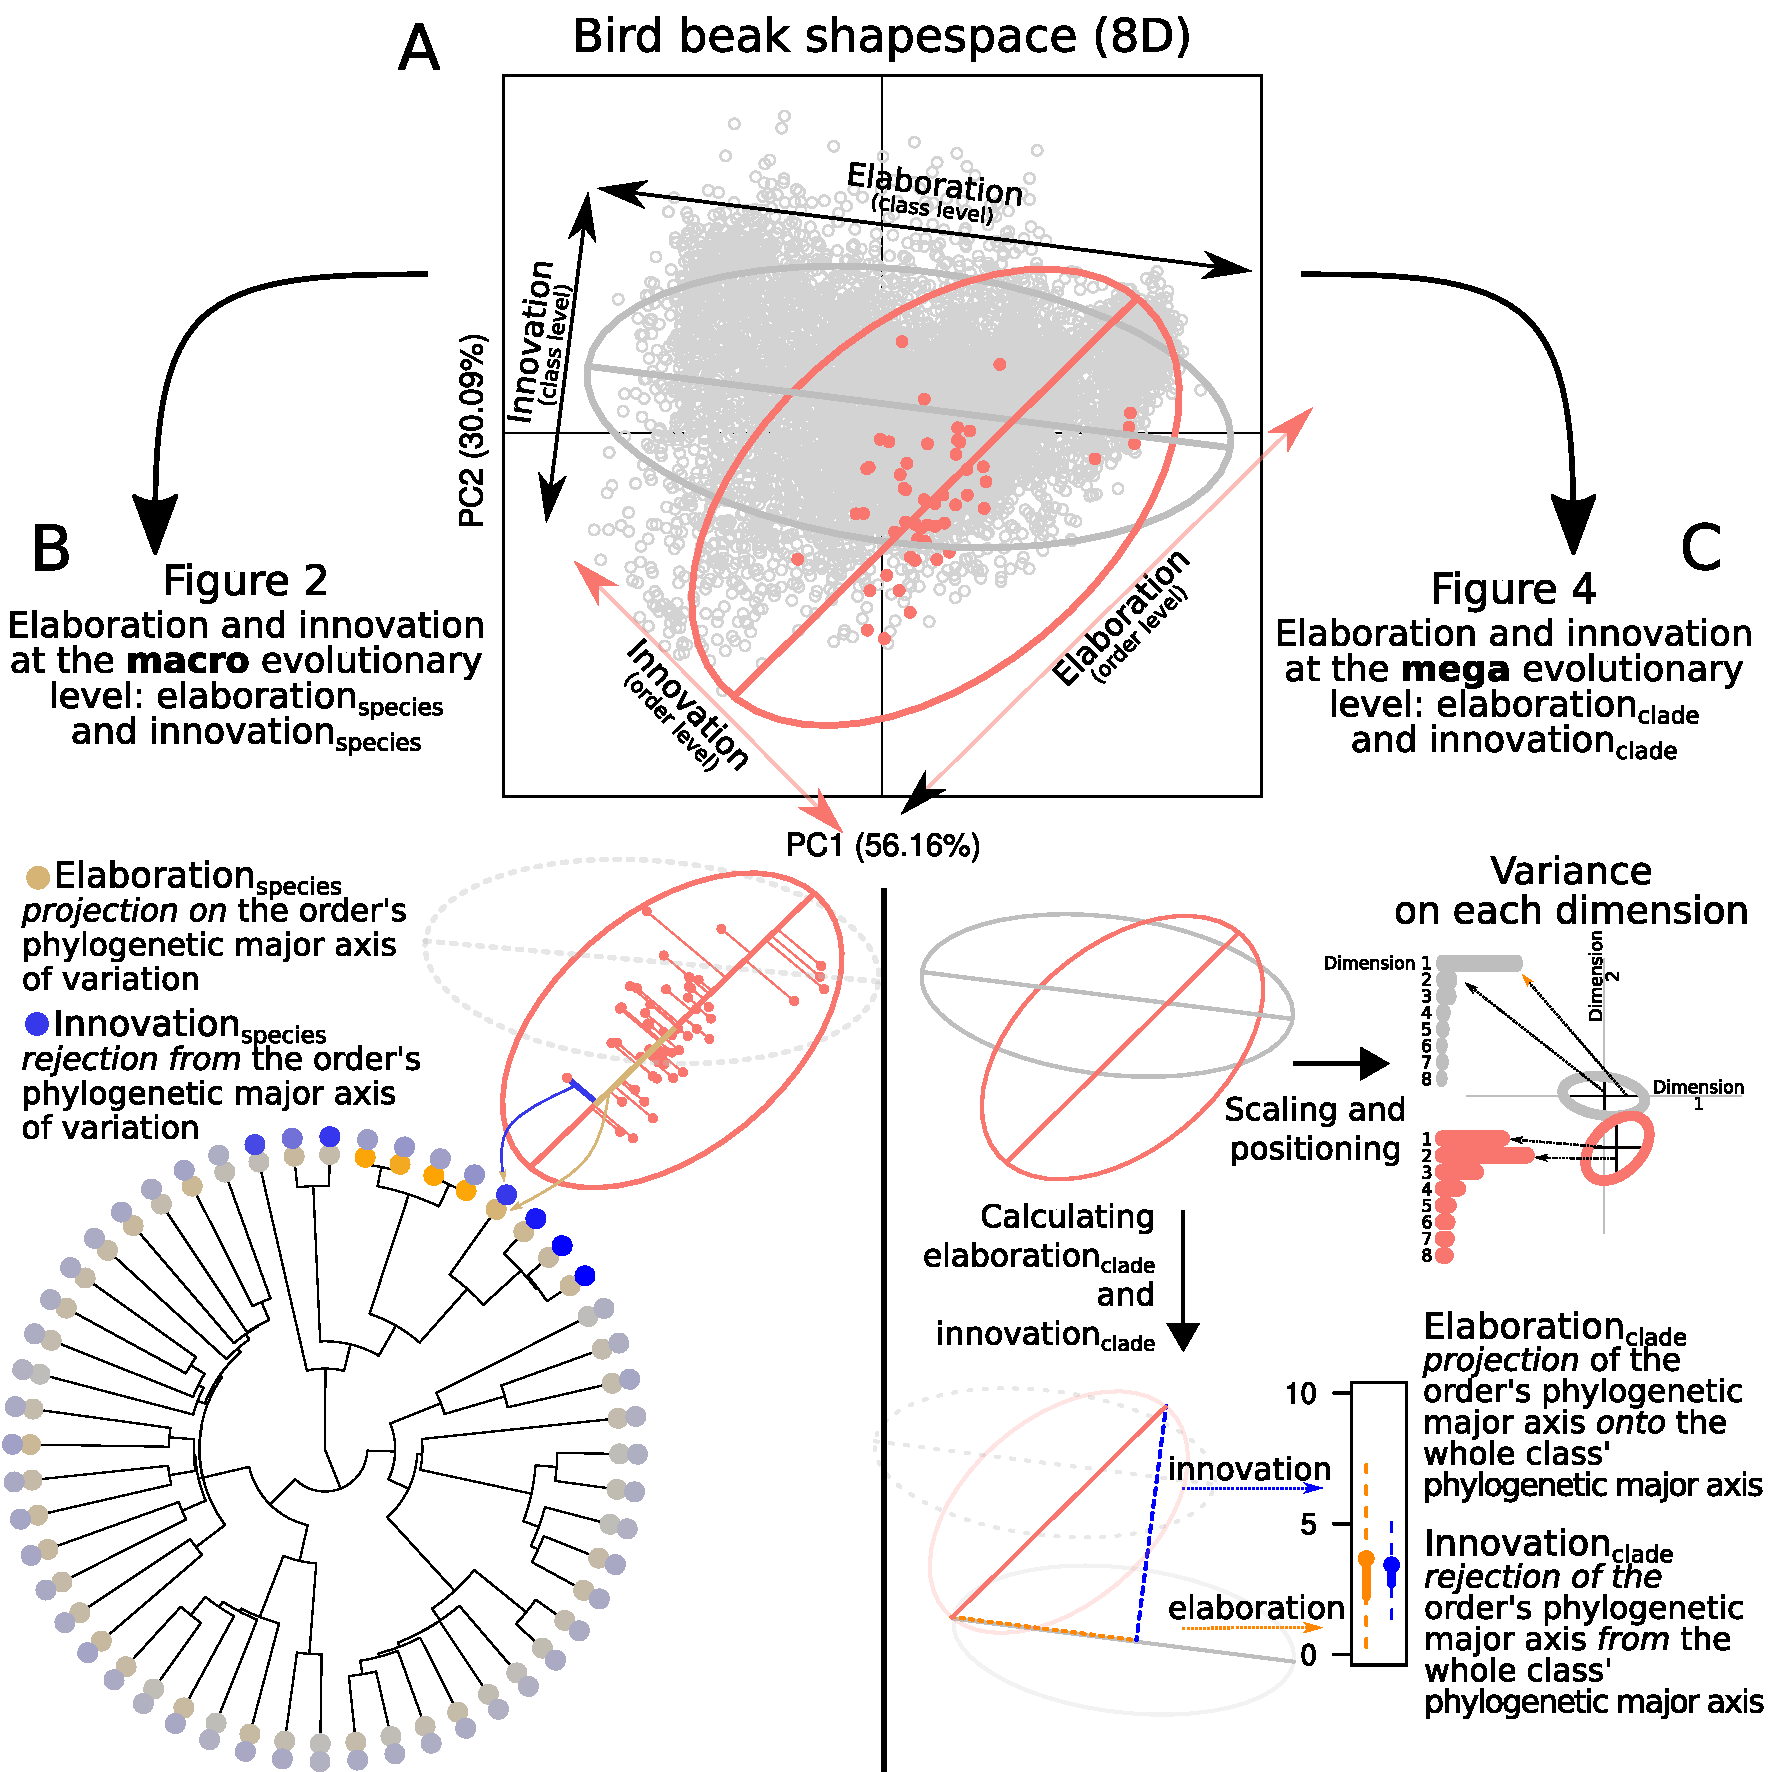
\includegraphics[width=0.6\textwidth]{Figures/cheat_sheet.pdf}
\caption{\scriptsize{Relationships between key figures in the main text.
A) represents the two first principal components (PCs) of the eight dimensional trait space with all bird beak shapes represented as gray circles and the Tinamiformes as red circles.
The gray ellipse represents the overall phylogenetic major axis of beak variation in birds.
Species aligned or away from this axis are respectively elaborators or innovators relative to the class Aves.
The red ellipse and axis represents the phylogenetic major axis of beak variation in Tinamiformes only.
Species aligned or away from this axis are respectively elaborators and innovators relative to the Tinamiformes order.
B) In Figure 2, we measured elaboration and innovation at the macroevolutionary scale , i.e. the position of each species in terms of $elaboration_{species}$ and $innovation_{species}$ relative to their order's phylogenetic major axis of beak variation.
A species $elaboration_{species}$ score is the species projection onto their order's phylogenetic major axis of beak variation(i. e. their position on that axis) whereas their $innovation_{species}$ score is their rejection from it (i.e. their distance away from that axis).
The colours on the tips of the phylogeny correspond to the median $elaboration_{species}$ (orange gradient) and $innovation_{species}$ (blue gradient).
C) Figure 4, we measured elaboration and innovation at the megaevolutionary scale, i.e. $elaboration_{clade}$ and $innovation_{clade}$.
The ellipses are scaled and centered and represent the clade's phylogenetic major axis of beak variation relative to the overall phylogenetic major axis of beak variation with the relative length of the ellipse on each dimension represented on the barplots as variance on each dimension.
A clade's $elaboration_{clade}$ and $innovation_{clade}$ scores are measured by projecting the clade's phylogenetic major axis of beak variation onto the overall phylogenetic major axis of beak variation and measuring the projection (elaboration) and rejection (innovation) from this axis as described above.
The distribution elaboration and innovation scores are taken from the projection of the 4000 pairs of evolutionary rate matrices with each pair being the focal level, e.g. order,and the parent level, e.g. the whole bird phylogeny.}}
\label{Fig:cheatsheet}
\end{figure}

\newpage

\textcolor{blue}{The abstract could benefit from briefly stating (e.g., a parenthesis) what innovation and elaboration are in this context. Similarly, the introduction would benefit from defining very clearly what is meant by micro- macro- and mega-evolution. I guess mega- in this context refers to divergence among major avian clades (order level or similar). Also bear in mind microevolution is within species so it is of limited utility here.}

We have now completely rewritten the abstract and introduction, ensuring we clearly introduce the concepts of innovation and elaboration, and mega-, macro- and micro- evolution. We defined the mega-, macro- and micro- evolutionary scales as the scales focusing respectively on the clades, species and individuals. We also link these concepts to the literature more thoroughly. Note that our previous version was a direct transfer from a journal with a more limited page count, but having more space to explain our approach has improved the manuscript substantially (lines 5-16):

\noindent\textit{Widely documented, megaevolutionary jumps in phenotypic diversity continue to perplex researchers because it remains unclear whether these dramatic changes can emerge from microevolutionary processes.
Here we tackle this question using new approaches for modeling multivariate traits %@L_multi_traits
 to evaluate the magnitude and distribution of elaboration and innovation in the evolution of bird beaks.
We find that elaboration, evolution along the major axis of phenotypic change, is common at both macro- and megaevolutionary scales whereas innovation, evolution away from the major axis of phenotypic change, is more prominent at megaevolutionary scales.
Indeed, the major axis of phenotypic change among species beak shapes at megaevolutionary scales is an emergent property of innovation across clades.
Our analyses suggest that the reorientation of phenotypes via innovation is a ubiquitous route for divergence that can arise through gradual change alone, opening up new avenues for evolution to explore.}

\textcolor{blue}{Lines 104-105: ‘We find no consistent evidence that innovation is either positively correlated, or trades-off, with elaboration’. Have you formally tested this? Maybe it would be good to show a dot plot of this for species values.}

We have now added a new analysis to the supplementary materials where we show the correlation between $innovation_{species}$ and $elaboration_{species}$ and we link to this figure in the main text (Figure 3). We find some variability in this relationship depending whether innovation and elaboration are calculated from comparisons to orders, suborders, or the whole tree. At the order level (our main focus in the new version of the manuscript) we find that positive correlations are common and negative correlations (trade-offs) are absent.


\begin{figure}[!htbp]
\centering
   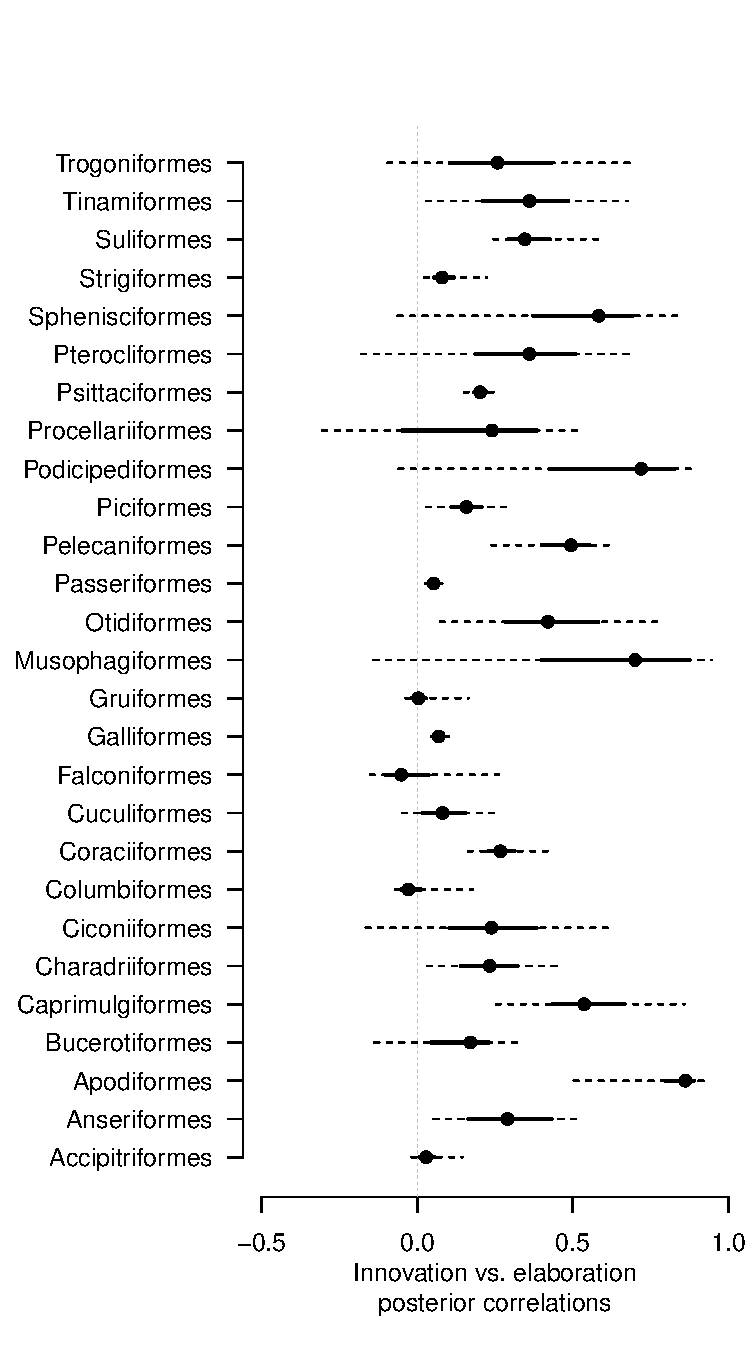
\includegraphics[width=0.5\textwidth]{Figures/correlations_fable_orders.pdf}
\caption{Posterior correlations between $elaboration_{species}$ and $innovation_{species}$ for each super-order. The dots, thick lines and dashed lines represent respectively the median, 50\% confidence interval (CI) and 95\% CI scores. 14 out of 27 of the orders have a clear posterior correlation between $elaboration_{species}$ and $innovation_{species}$ (i.e. 95\% CI does not overlap with 0), nine have a somewhat positive posterior correlation (i.e. 50\% CI does not overlap with 0) and four have no clear posterior correlation. Note that no order has a clear negative posterior correlation. This trend suggests that there is no tradeoff between $elaboration_{species}$ and $innovation_{species}$ and that both can be common routes for beak shape evolution at the macroevolutionary scale.
}
\label{fable_correlations}
\end{figure}
\bigskip

\newpage

\textcolor{blue}{Overall, I think the Results are written in a slightly disorganised and convoluted way (e.g., lines 91-94) and that could be easily improved.}

We have re-written the results, and reframed the manuscript to only focus on $elaboration_{species}$ and $innovation_{species}$ projected on their order’s major axis. e.g. lines 158-162:

\noindent{We found typically higher values of $elaboration_{species}$ than $innovation_{species}$ (Fig. \ref{Fig:phylogeny}) %@L_rephrase_wefound
and strong clustering of both $elaboration_{species}$ and $innovation_{species}$ (median $elaboration_{species}$ for all orders = 0.114, 95\%CI = 0.004-0.485;  $elaboration_{species}$ Pagel's $\lambda$ = 0.888; median $innovation_{species}$ for all orders = 0.071, 95\%CI = 0.018-0.224); $innovation_{species}$ Pagel's $\lambda$ = 0.848).%@L_ei_species_values. }


\textcolor{blue}{Figures:
I think the figures can be significantly improved. I personally feel it would be a pity that this important study will go unnoticed because the figures are less intuitive or aesthetic than they could be, so, I suggest that the authors could put a bit more emphasis on trying to make them easier to read.}

We have improved and modified our figures as suggested below, so hopefully they are now more intuitive.

\textcolor{blue}{Figure 1:Considering colours carry meaning in this figure I suggest removing clade colours and using alternate shades of grey or of one single hue as per Cooney, Bright et al., 2017, for instance. Some silhouettes for each major clade could better guide the readership.
I also suggest using one palette for innovation and another one for elaboration. These palettes would ideally go from grey for low values to a single hue for high values (e.g., orange for innovation; blue for elaboration).}

We tried adding silhouettes to the former figure 1 (now figure 2; circular phylogeny) however, due to the imbalance in clade sizes, the silhouettes are either mostly clumped in one portion ofthe tree due to the dominance of the passerines which looks unpleasant, or if they are spread evenly they are not next to the correct clade which is misleading. Therefore we have chosen to omit silhouettes but have overall simplified the figure. We do this by removing the innovation and elaboration scores for the whole phylogeny and the super-orders and standardised innovation and elaboration colour gradients as suggested (this was a really good suggestion, thanks). We have now changed the colour coding throughout the manuscript using orange for elaboration and blue for innovation. When showing gradients of either elaboration and innovation we are now using a gradient from grey (0) to orange/blue (highest value of elaboration/innovation) as suggested.

\textcolor{blue}{Some typos in the caption. Fix please. There is some text that is not very clearly written – check please.}

Fixed.

\textcolor{blue}{‘Blue and yellow colours on the branches of the phylogeny highlight species with relatively low distances to the global centroid of trait space whereas orange to red colours indicate high distance from the centroid’. In your figure the branch colours go from blue to yellow.}

Fixed.


\textcolor{blue}{Finally, I really do not understand the left boxplot inset.}

We have removed these boxplots altogether since we now only focus on the distribution of elaboration and innovation at the order level for the main text.

\begin{figure}[!htbp]
\centering
   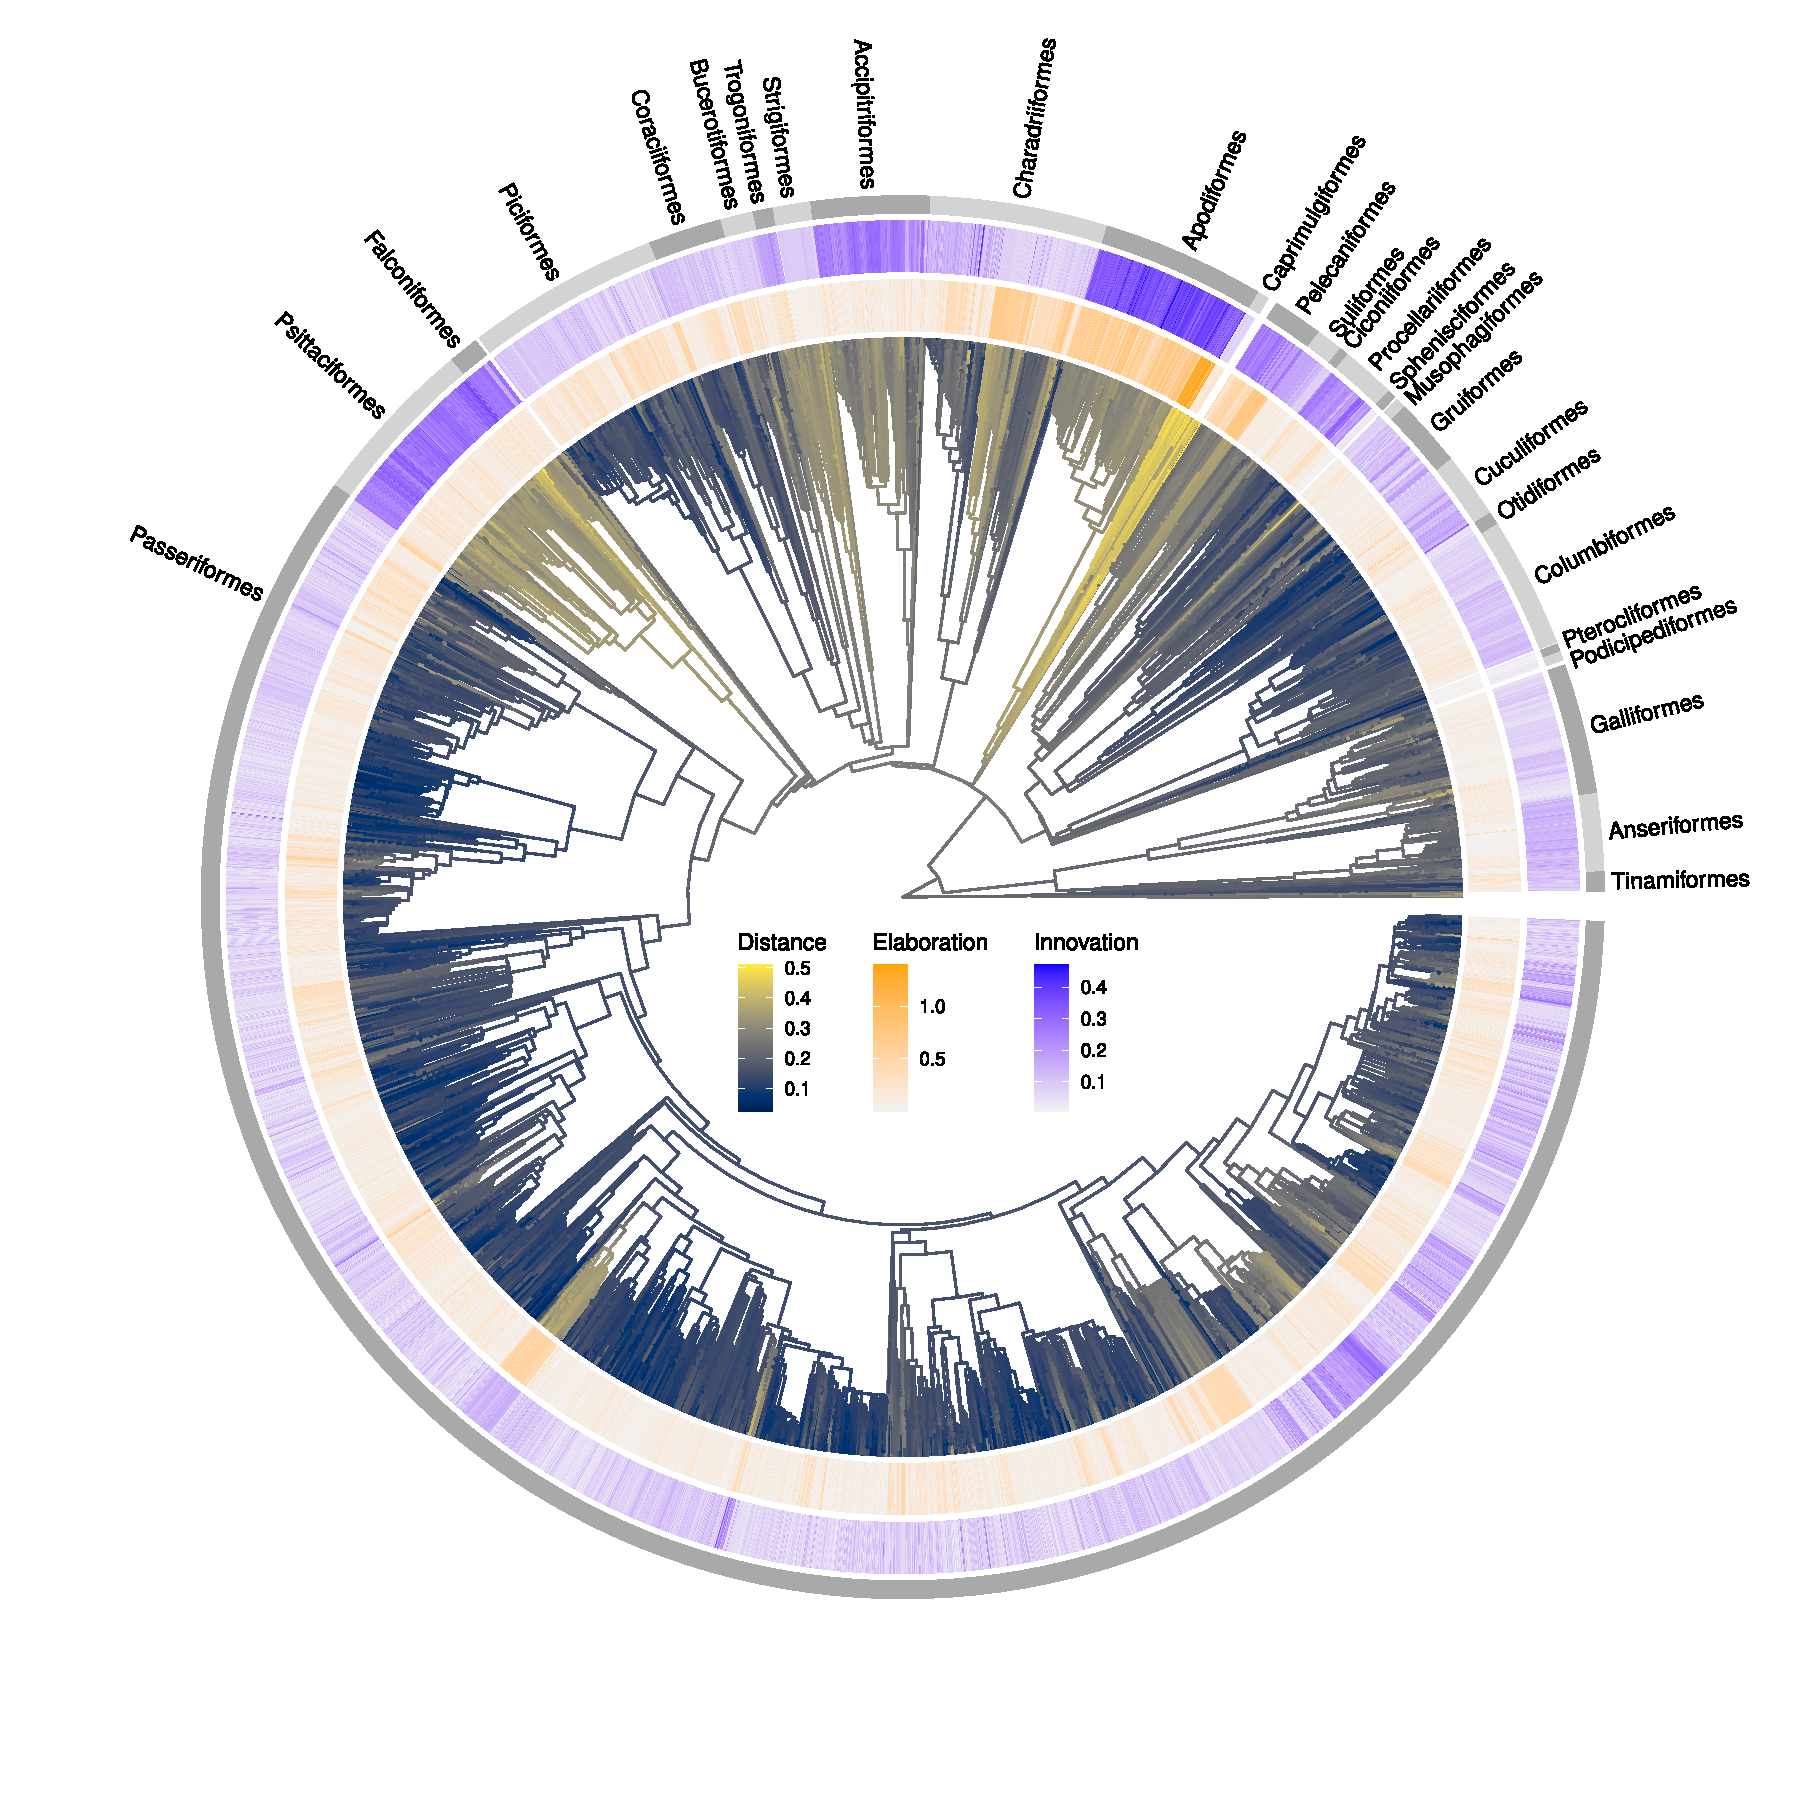
\includegraphics[width=0.8\textwidth]{Figures/InnovElabTree_main_text_revision.pdf}
\caption{Avian phylogeny (n = 8748 species) showing Euclidean distance of species to the centroid of beak space (branches, cividis scale), and distributions of species beak shape $elaboration_{species}$ (inner circle, orange scale), and $innovation_{species}$ (outer circle, blue scale).
Elaboration and innovation scores represent comparisons of species at the order level.
Additional comparisons to super-orders and at the class-wide phylogenetic level are shown in Fig. \ref{Fig:phylogeny_supplement} and for family and super-family comparisons of the order Passeriformes in Fig. \ref{fig_phylogeny_passeriformes}.
}
\label{Fig:phylogeny}
\end{figure}
\bigskip

\textcolor{blue}{Figure 2: I think you could use another colour that shows better contrast among each other perhaps using a palette which is not the default from ggplot. Also please label elaboration and innovation in the boxplots by each clades plot.}

The colour palette used here is not from ggplot (although we agree it looks very similar) and was chosen to offer the maximum contrast gradient among lineages. However, we agree that it is difficult to discern the different colours (it’s hard to find a palette for 35 nested variables!), so we have removed the colours from this plot. We have also completely reworked figure 2 (now figure 3) so it is now presented in a phylogenetic format with the super-orders overlapping the orders. We have also standardised the colours for elaboration (orange) and innovation (blue) as suggested in the comment about figure 1 above.

\newpage

\begin{figure}[!htbp]
\centering
   \includegraphics[width=0.6\textwidth]{Figures/figure_phylo_spiro_dark.pdf}
\caption{\scriptsize{$Elaboration_{clade}$ and $innovation_{clade}$ at the megaevolutionary scale for each order and super-order in the bird phylogeny.
The black and gray ellipses are the scaled average evolutionary rate matrices from the pGLMM models for respectively the clades (black) and the class-wide phylogeny (gray).
The ellipses are centered on the position of the clade in the shapespace.
The associated black bar plots represent the variance on each of the eight dimensions in the shapespace with the top gray bar plot representing the variance on each of the eight dimensions for the class-wide phylogeny.
The orange and blue distributions represent respectively the distribution of the $elaboration_{clade}$ (orange) and the $innovation_{clade}$ (blue) scores for each clade and the dots are the median $elaboration_{clade}$ or $innovation_{clade}$ and the solid and the dashed lines representing the 50\% and the 95\% confidence intervales of the distribution of the scores across the 4000 posterior samples.
The ticks on the y-axis always represent five arbitrary units of elaboration and innovation.
An alternative visualization of the same information is available in the supplementary materials in Fig. \ref{Fig:ellipses_rainbow} along with a companion plot showing further nested structure within the Passeriformes in Fig. \ref{fig_ellipses_passeriformes}.}
}
\label{Fig:ellipses}
\end{figure}

\newpage

\textcolor{blue}{Figure S5 caption: ‘The distribution of innovation and elaboration scores comes from the projection of the 4000 pairs of posterior VCVs.’ It would be good to briefly state where these 4k pairs are.}

We have now integrated Figure S5 into the main text (as figure 1) and have completely rewritten the caption (including the precision of what these pairs are). See comment above referring to now figure 1:


\noindent\textit{Relationships between key figures in the main text.
A) represents the two first principal components (PCs) of the eight dimensional trait space with all bird beak shapes represented as gray circles and the Tinamiformes as red circles.
The gray ellipse represents the overall phylogenetic major axis of beak variation in birds.
Species aligned or away from this axis are respectively elaborators or innovators relative to the class Aves.
The red ellipse and axis represents the phylogenetic major axis of beak variation in Tinamiformes only.
Species aligned or away from this axis are respectively elaborators and innovators relative to the Tinamiformes order.
B) In Figure 2, we measured elaboration and innovation at the macroevolutionary scale , i.e. the position of each species in terms of $elaboration_{species}$ and $innovation_{species}$ relative to their order's phylogenetic major axis of beak variation.
A species $elaboration_{species}$ score is the species projection onto their order's phylogenetic major axis of beak variation(i. e. their position on that axis) whereas their $innovation_{species}$ score is their rejection from it (i.e. their distance away from that axis).
The colours on the tips of the phylogeny correspond to the median $elaboration_{species}$ (orange gradient) and $innovation_{species}$ (blue gradient).
C) Figure 4, we measured elaboration and innovation at the megaevolutionary scale, i.e. $elaboration_{clade}$ and $innovation_{clade}$.
The ellipses are scaled and centered and represent the clade's phylogenetic major axis of beak variation relative to the overall phylogenetic major axis of beak variation with the relative length of the ellipse on each dimension represented on the barplots as variance on each dimension.
A clade's $elaboration_{clade}$ and $innovation_{clade}$ scores are measured by projecting the clade's phylogenetic major axis of beak variation onto the overall phylogenetic major axis of beak variation and measuring the projection (elaboration) and rejection (innovation) from this axis as described above.
The distribution elaboration and innovation scores are taken from the projection of the 4000 pairs of evolutionary rate matrices with each pair being the focal level, e.g. order,and the parent level, e.g. the whole bird phylogeny.}


\section*{\textcolor{blue}{Reviewer 2}}

\textcolor{blue}{I appreciate what the paper is trying to quantify, and find the topic quite interesting. Obviously the dataset is stupendous. I support continued consideration of the ms. However, at present it is very confusing. Terms are used inconsistently and the link between analysis and hypotheses is not laid out with sufficient clarity (other than the authors stating that their method is 'powerful'). The text is too short, and there does not seem to be any reason why it must be so concise. It does not place the work in a broader macroevolution context, or speak to the fact that birds are real biological entities that are a field of study in their own right. I am also concerned that the ms as currently written is very confusing, will not speak to a wide audience, and has a great deal of opacity around the methods and concepts. In its current form therefore it is a highly technical piece for a more specialist journal. However, the authors have a lot of scope to improve on this. The work has a great deal of potential and I would like to see the review process continue.}

\textcolor{blue}{I hope that my comments below are useful to the authors in pursuing this. Sorry that I have written so much. I have also made suggestions that may result in changes to the analytical approach. My intention is to be as clear and constructive as possible and I hope that the authors find this helpful.}

Thanks for these comments. Note that in our previous version was written for Science and was transferred to Science Advances without modifications. We fully take advantage of having more space to explain our approach which has improved the manuscript substantially. We detail our changes below.

\subsection*{\textcolor{blue}{Major comments}}

\textcolor{blue}{(1) The methods used assume that the evolutionary lines of least resistance are univariate, and can be derived from data at high taxonomic levels, with some biological meaning. The interpretations start are on soft ground if we thought there might be causes for bivariate or multivariate lines of least resistance at high taxonomic levels. Or even that lines of least resistance inferred at higher taxonomic levels did not have a straightforward biological interpretation. Myself, I'd be a lot more confident in the hypotheses that there are evolutionary lines of least resistance at low taxonomic levels (i.e. among closely related species), but I'm not sure what to make of this hypothesis at high taxonomic levels. Therefore it is challenging for me that the analytical procedure starts with higher-level patterns and interprets lower level pattern in light of those, and not vice versa. The procedure in which major axes of variation for subclades or phenotypic data for species are compared to the whole clade of all birds seems to run backward compared to the reasoning derived from theory. It isn't clear that this means what the authors say it does. The underlying theory seems to be that there are evolutionary lines of least resistance at more local phylogenetic scales (e.g. within a group of closely-related species), and that the morphological variation resulting from shifts in these could be interpreted as innovation. This suggests a procedure that compares patterns among similar-level groups, or compares the patterns at larger phylogenetic scales to the predictions of extrapolating what was found at smaller scales. It may be that the procedure can be done backwards and yield equivalent, interpretable, results. But this needs to be unpacked and explained clearly. I'm concerned about this (see point (1) above).
Within the current set of analyses, the analysis I find the most useful is the one that compared major axes ('lines of least resistance') among subgroups of approximately equivalent rank, finding them to be generally different to each other. However, this needs development (see my detailed comments) because currently there are unsupported statements such as the statement that evolution can happen in 'any' direction.}

Some of this is related to misunderstandings about our method and how it builds on the previous literature. This was our fault for not fully explaining things in the introduction and we hope we have now explained things more clearly.

First, we chose to work with univariate evolutionary lines of least resistance rather than surfaces or volume because we believe they are more correctly interpreted as directional vectors in any number of dimensions. For example, classically, adaptive landscapes are represented in two dimensions with a third dimension being the theoretical fitness advantage from the covariance between the two said dimensions (e.g. as illustrated here: \url{https://en.wikipedia.org/wiki/Fitness_landscape}). In this context the line of least resistance is the vector pointing towards peaks in the landscape. This has the advantage of working with any number of dimensions (whereas a surface or volume are bound to at least n+1 dimensions) and remains interpretable by biologists (i.e. the ``evolutionary direction'').

Second, evolutionary lines of least resistance are by their nature designed to investigate patterns across higher-levels. However, we agree with the reviewers’ comment that this might be confusing in this specific manuscript. We have thus narrowed down the taxonomic levels presented in the main text and are now only focusing on the $elaboration_{species}$ and $innovation_{species}$ projected on the the eigenvalues of the order’s evolutionary rate matrix which we interpret as similar to lines of least resistance at the micro-evolutionary scale. We have now clarified this throughout the manuscript. E.g. on lines 52-60:

\noindent\textit{At this scale the major axis of phenotypic variation among species \cite{marroig2005size, fasanelli2022allometry} can be estimated from a matrix of divergences in species mean phenotypic traits (e.g. the \textbf{D} matrix of \cite{BlowsHiggie2003, mcglothlin2018adaptive}.
These matrices do not take into account phylogenetic relationships among species.
In contrast, the \textbf{R} matrix of \cite{Houle2017} describes the rate of among-species divergence in species traits and explicitly incorporates phylogeny (also see the \textbf{B} matrix of \cite{Machado2020}) %@L_Rmatrix.
We hereafter refer to this \textbf{R} matrix as the \textit{evolutionary rate matrix}. %TG: TODO: change throughout (that's the VCV matrix now)
The major axis of the evolutionary rate matrix is a phylogenetic line of least resistance applicable at macro- and mega-evolutionary scales that is analogous to the genetic line of least resistance at microevolutionary scales. }

\textcolor{blue}{(2) The paper is notionally quantitative. And is quite abstract and complicated in the way it was written. But actually, under the surface, a lot of the interpretations are actually qualitative (see several of my comments where I have requested to report a qualitative test of hypothesised interpretations). This should be avoided where possible.}

We acknowledge that some interpretations are qualitative. However, these are based on detailed quantitive analysis generating large posterior distributions of parameter estimates. We have now added references to more supplementary figures providing the exact values from our analyses where appropriate. In the revised main text, Figures 3, 4 (part), 5, and 6, and the new Table 1 provide explicitly quantitative analysis. See details below for further analyses added to the text. We have also improved the clarity of the writing which hopefully helps highlight our quantitative findings.

\textcolor{blue}{(3) A major conclusion is that "Species elaborate, clades innovate". But the difference between species and clade is an arbitrary one. Species are just the arbitrary subset of evolving lineages that cross the present-day time horizon. They have the attribute of being highly over-sampled compared to lineages that occur deeper in the phylogeny. Please envision an unfolding evolutionary process generating phenotypic variation through time. Let's say that 'innovation' by your definition is rare, but makes a directional and general unreversed change (these off-axis changes should be difficult to reverse by chance because we have a wide range of off-axis trait changes we could make so the chance of randomly drawing the 'right' one is low). Int he same process, 'elaboration is common', and is also 'easy' to reverse because it occurs along one univariate axis. If we sample information about a high proportion of lineages alive at some particular time (the present) then we expect to find that the differences between species phenotypes mainly reflect elaboration. But if we sampled fewer, then the difference between species phenotypes will reflect an increasing contribution of innovation. I don't think this a. Big problem for the analyses oft he paper. But I think ti is a problem for the interpretation that arbitrarily- designated taxonomic ranks are important. This rank-based, interpretation makes the present-day into a 'special' time and has little meaning in terms of the evolutionary process.}

We have now nuanced this subtitle by changing it to the following (line 293):

\noindent{\textit{Species elaborate \textit{and} innovate, clades innovate}}

Furthermore, we agree with the reviewers comment on how clades and species are arbitrary cuts of a continuum, they do, in our view, however remain a common and useful tool in research to understand evolutionary biology \cite{baker2021nothing}, particularly in well studied taxa such as birds where high taxa map meaningfully to phylogeny and trait variation. As the reviewer notes, it is possible that the major axes change depending on the specific bracketing of taxa (as would be true using arbitrary timescales). However, here we use two different higher taxonomic levels for comparison and find broadly consistent results when taken together. One additional strength of a taxonomy based approach is that it doesn’t force arbitrary time constraints on interpretation. Indeed, the higher taxa that we focus on span a wide range of timescales. This has enabled us to conduct new analysis (inspired by the reviewers comments) in the supplementary materials showing the distribution of $elaboration_{species}$, $innovation_{species}$, $elaboration_{clade}$ and $innovation_{clade}$ through time. This new analysis indicates that the magnitude of both elaboration and innovation increases with time since divergence, as would be expected under the commonly used Brownian motion model of evolution. lines 242-243: %@L_ei_through_time_plots

\noindent\textit{Similarly, when measured at the macroevolutionary scale, $innovation_{species}$ and $elaboration_{species}$ increase with species age (see supplementary Fig. \ref{Fig:figure_ei_clade_through_time} and \ref{Fig:figure_ei_species_through_time}). }%@L_ei_through_time_plots}

\textcolor{blue}{(4) The ms includes very few citations and is broadly not in conversation with the wider literature. The approach and its conclusions come across as being very abstract in nature. Let's keep a sense of perspective here, the work is about birds, but only a very selective subset of work on bird evolution is cited, primarily by the group who wrote this paper. A lot more could be done to make this work accessible to a wide audience, not only for biologists interested in birds, but also for wider macroevolutionary study. For example, how do the approaches used here connect with other forms of inference? The conceptual framework used here maid numerous references to Endler et al (2005), as though nearly two decade since then provided no useful ideas. It may be true that there has not been much specific, directed work that formalises the concepts of innovation or elaboration. Nevertheless, many other works contain relevant analyses and interpretations and the authors here show little attempt to integrate those works in their synthesis. The contributes to the impression of an opaque and abstract study with little reach.}

We have now updated and added many more references throughout the whole manuscript (from 28 to 63), expanding on the background and giving more context to the Endler et al study. Our previous version was a direct transfer from a journal with a more limited page count so we have been able to fully make use of the available space to expand our ideas, citations and links to the existing literature.


\textcolor{blue}{(5) There are some confusing and inconsistent uses of terms (see my detailed comments). Sometimes it seems like unnecessarily elaborate language is used, compounding the issues. For example:}

\textcolor{blue}{ -'Shapespace' would just be 'shape' in most studies. 'Shape' is more appropriate in the statistical model formula because each taxon has 'shape', but does not have 'shapespace'.For example, you wouldn't write out "skull size range $\sim$ body size range", you'd write "skull size $\sim$ body size".}

We respectfully disagree with this comment. Although the reviewer is right that most studies would use the term “shape”, we do like the precision that the term “shapespace” adds to the formula (the correct most precise term would be “position of species in the shapespace”). 
We do make the distinction that a single species beak has a shape (the raw data from the bird beaks, described using classic gmm approach) and that the shapes of multiple species beaks occupy a shapespace (the transformed and usable data for our analyses after Procrustes superimposition, ordination and dimensionality reduction - lines 363-378). In the skull/body size example provided by the reviewer, naming the terms “skull size range” might actually bring a useful methodological precision (what is the skull or body size) while simply using “skull size” gives the more general idea (comparing the skull to the body size). In our case, since the formula is in the methods section, we chose to emphasise the methodological aspect rather than the general aspect.

\textcolor{blue}{-'Multilinear algebra', is more typically called 'linear algebra'. In fact, it would be better to say what computation was performed e.g. taking the dot product or cross product, or whatever. Here, little attempt has been made to clearly communicate what is being done.}

We have changed multilinear algebra to linear algebra throughout the manuscript. The whole mathematical procedure can be found in the supplementary materials. We have now specified that in the main manuscript along with the previous brief description of what computation was performed (projection). lines 154-158:

\noindent\textit{To assess this we projected the beak shape data for each species onto %@L_linear_algebra_stuff @L_beak_shape
the major axes of evolutionary rate matrices of their orders (see supplementary materials \ref{Fig:phylogeny_supplement} for projection onto the major axes of beak shape variation from the class-wide phylogenetic major axis of beak variation or their super-order’s phylogenetic major axis of beak variation).}

\textcolor{blue}{-"Species phenotype' is used in many places where the 'beak shape' is actually being referred to. The 'phenotype' is all the morphological and behavioural traits of an organism. Not just the beak shape. It is OK to call it 'phenotypic data', but not 'species phenotype'.}

We have changed “species phenotype” to “species beak shape” throughout.

\textcolor{blue}{(6) Choice of nodes to analyse - order and suborders represent an arbitrary subset of nodes on the tree. Is there a justification for not analysing patterns across all pairs of ancestor and descendent nodes in the full tree? This is important because something the patterns for e.g. orders are compared to each other as though they were meaningful biological units that could be expected to share some features. In fact, they cannot.}

We agree that the choice of nodes to analyse is ultimately an arbitrary decision (see our comment above). We had originally considered analysing every node and agree this would be great. However we decided to use the named nodes (orders and super orders) for the following reasons:
\begin{itemize}
\item We estimate that it would take between 5 CPU centuries + 1ZB of RAM (using the normal MCMCglmm framework) or 12 CPU millenia + 2.5 GB of RAM (using the mcmcmcglmmm framework). Both are currently not achievable with modern computers.
\item Named nodes represent divergence points of interest to biologists (especially ornithologists) and are based on common biological features shared by living species within the orders (namely their beaks).
\end{itemize}

We’ve added a plot of $elaboration_{clade}$/$innovation_{clade}$ through time per clade (orders and super-orders) to the supplementary materials to give an idea of the time span of the named nodes used in the analysis and how it might affect our results. This plot gives a rough idea on how the nodes are distributed through time (lines 242-243).

\noindent\textit{Similarly, when measured at the macroevolutionary scale, $innovation_{species}$ and $elaboration_{species}$ increase with species age (see supplementary Fig. \ref{Fig:figure_ei_clade_through_time} and \ref{Fig:figure_ei_species_through_time}). }%@L_ei_through_time_plots}


\textcolor{blue}{(7) The interpretations emphasise 'levels' of innovation and elaboration. But these absolute amounts cannot be interpreted easily, independent of the total amount of phenotypic variation for a (arbitrarily delimited) subgroup. I'd like to see more transparency about variation the relative importance of each of these effects among groups.}

We are not sure about what the reviewer means by “transparency” in this context. Figure 3 shows the distribution (including the 50 and 95\% CI) of the posterior distribution of the $innovation_{clade}$ and $elaboration_{clade}$ scores. The code and the data to reproduce this figure is made available on GitHub \url{https://github.com/TGuillerme/elaboration_exploration_bird_beaks}. We have now also added a whole new analysis where we test how the amounts of elaboration and innovation relate to overall beak divergence using PGLS models presented in the new Table 1. (lines 311-324)

\noindent\textit{We further tested the contributions of elaboration and innovation at different scales by examining the consequences of elaboration and innovation for the observed divergence of bird beak shapes. Specifically, we calculated the distance to centroid of avian beak morphospace for each species (Fig. \ref{Fig:phylogeny}).
We then used phylogenetic generalised least squares (PGLS; \cite{phylom}) to model distance to centroid as a function of $elaboration_{species}$, $innovation_{species}$ and $elaboration_{clade}$ and $innovation_{clade}$.
We ran the PGLS analysis using both single and multiple predictors.
Our analyses indicate that the majority of variation (r2 = 0.888; Table 1) in beak shape centroid distance can be explained by a combination of $elaboration_{species}$ and $innovation_{species}$.
When modeled as single predictor models, variation explained is lower for $elaboration_{species}$ than $innovation_{species}$ and $innovation_{species}$ has a steeper slope indicating that although elaboration is overall the dominant model of divergence, innovation leads to greater exploration of morphospace (Table 1).
In contrast, the combination of $elaboration_{clade}$ and $innovation_{clade}$ alone explains only $>$0.01\% of the total variation in beak shape divergence (Table 1).
However, $innovation_{clade}$ is nonetheless an important contributor to total beak shape space.
We reach this conclusion because models with interactions between species and clade metrics provide by far the best model fit overall and removal of terms indicate that the most important interactions are between $innovation_{clade}$  and $innovation_{species}$ followed by $innovation_{clade}$ and $elaboration_{species}$.
The interaction terms show that the relationship between species metrics ($elaboration_{species}$, $innovation_{clade}$) and distance to centroid becomes steeper as $innovation_{clade}$ increases (Table 1)
Overall, the models suggest that although most species evolve via elaboration at the macroevolutionary scale, expansions of beak morphospace are also driven by megaevolutionary scale reorientations of trait space.
}

\textcolor{blue}{(8) The authors choose a computationally-intensive method to find the major axis of variation, and then say they can't do more because of computational intensity. But the decision to take this approach in the first place is not explained. It also isn't clear that the mini-chains or the aggregate result from them has converged because no info about convergence is given. Could their be come comparison to a similar method that requesters less computation power such as phylogenetic PCA, that may validate that the major axes returned are sensible?}

We use the mini-chains approach to account for phylogenetic uncertainty. Our phylogenetic hypothesis comes from a Bayesian analysis so it is not appropriate to perform analyses on just one tree. Therefore a posterior distribution of trees needs to be used. This is not possible within our basic MCMCglmm format without a huge amount of computational time, thus we developed the mini chains approach to make it tractable. Phylogenetic PCA would not provide a solution to this issue as it also uses one tree, nor can it provide results in a nested way as our method does. We have now added a clearer explanation of why the mini chains were used.

We do not provide convergence information between mini-chains since they are considered in our framework as different samples from the same chain. We are thus effectively running single chains for each of the 35 nested clades. Running pairs of chains would just double the amount of computational time and not provide useful information. In fact, this mini-chains method highly favors accuracy over precision, therefore mini-chains with a high level of uncertainty (e.g. because of a small clade size) will always lead to imprecise but accurate results (i.e. two blurry posteriors). This means that convergence will never be useful information as some of the chains will be not converging on anything by design (i.e. the “true” precise solution is unknown but the 95\% posterior accurately contains the “true” solution). We do however include the distribution of effective sample sizes for all chains (supplementary information S3 and S4) which gives a good indication of the posterior distribution containing enough samples to be used as the “true” solution. Note that for all analytical parts in the analysis, we use the entire posterior distribution - we only use the averages from these distributions for plotting and in the new PGLS analyses. We have added this precision in the manuscript (lines 450-454).

\noindent\textit{The full mathematical procedure is described in detail in the supplementary materials (section \ref{supp_projection} - note that the procedure described in the section \ref{supp_projection} is applied to each individual evolutionary rate matrix for each term in the model, e.g. for each 4000 posterior variance matrices individually for each $elaboration_{species}$, $innovation_{species}$, $elaboration_{clade}$ or $innovation_{clade}$ score. %@L_individual_matrices).
}


\subsection*{\textcolor{blue}{Detailed comments}}

\textcolor{blue}{Abstract}

\textcolor{blue}{Lines 7-8: "Here we reconcile major changes in phenotypic diversity at macroevolutionary scales with gradual microevolutionary change"
>>I read the ms a few times, considering whether the approach used here reconciles the patterns at smaller scales with those at larger scales. I think it is a descriptive method rather than a model of varying processes at different scales. So I'm not comfortable with the statement that it 'reconciles' these things. That reconciliation is done int h msusing verbal argument - and this verbal arguments are based on a much older literature. Consider re-phrasing here.}

We have now reworded the abstract without “reconcile”.

\textcolor{blue}{Lines 8-9: "using new multi-trait models"
$>>$It isn't clear that these are 'multi-trait models' rather than 'approaches to modelling multivariate traits'. The subject of the current study is beak shape, which arguably is a single multivariate trait rather than multiple traits (implied by 'multi-trait').}

We’ve changed “new multi-trait models” to “new approaches to modelling multivariate traits” as suggested. (line 8)

\textcolor{blue}{Lines 10-11: "We find that elaboration dominates at macroevolutionary scales whereas innovation becomes more prominent at megaevolutionary scales"
$>>$I quite like these terms 'mega' and 'macro'. But we should probably acknowledge that the distinction is qualitative and arbitrary. Here, it would be more useful to directly state the taxonomic scales of the analyses. That is avoids going too far down the road of abstraction.}

Following this reviewer’s previous comment on arbitrariness, we do agree but find this comment inapplicable (everything we do is arbitrary). Also we disagree on the absence of distinction between “mega” and “macro”, we refer here to “macro” as the species focal level (i.e. using species rather than individuals as the unit of our analyses) and “mega” as the clade level (i.e. using groups of species rather than individual species as the unit of our analyses). We have now specified this one lines 82-83

\noindent\textit{The phylogenetic breadth of the data allows us to compare directions of beak evolution of subclades (e.g. orders) within the class Aves (the megaevolutionary scale) and of species within subclades (the macroevolutionary scale).}%@L_macromega_definition2

\textcolor{blue}{Introduction}

\textcolor{blue}{Lines 24-27: "However, while the evolutionary line of genetic least resistance explicitly reflects genetic constraints, the macroevolutionary major axis of phenotypic variation is an emergent property of genomic and developmental constraints interacting with selection on a moving adaptive landscape"
$>>$Some inconsistency of language in these statements. The first clause says 'genetic' and the second clause say 'genomic and developmental'. I think that the authors are referring tot he same identical thing twice, but using different words each time. If so, please make this consistent so it is easy for a reader to follow your meaning.}

We have now entirely rewritten the introduction (also following the other reviewers comments). 

\textcolor{blue}{Lines 31-33: "Resolving this conflict requires an understanding of the balance between deep-time reorientation of phenotypic major axes of evolution among clades and the directions of evolution of species within clades"
$>>$"Balance" here is a metaphor and is potentially confusing. Consider something like "the relative contributions of ..."
$>>$I also think it is important to say that what they are contributions towards. I suspect you are asking about the relative contributions of these conceptual processes to the total disparity of a large group such as all birds. If so, can you clarify this here, and potentially in other places where this important goal of the study is stated.Lines 41-43: "Relative to elaboration, innovation may be more likely to generate phenotypic novelty, but this need not be synonymous with being a primary driver of phenotypic diversity at broad scales"
$>>$There is first-pass evidence relevant to this across many fields of evolutionary research (e.g. paleontological study of major evolutionary transitions; island biogeography; developmental biology; many others). Only one area is mentioned (signal evolution), and that relies on one citation from 2005. It seems strange to me that the authors have this pinpoint focus on one item of literature. It makes the while topic seem a lot more esoteric and erudite the it actually is. Could the authors please contemplate broadening their introduction into a wider biological context. The work should be integrative rather than striking out in a unique direction with undue emphasis on one paper from 2005.}

We have now entirely rewritten the introduction (also following the other reviewers comments) to make our motivations clearer. We used the Endler et al. (2005) paper as inspiration for the ideas of innovation and elaboration (hence the focus on a single paper) but acknowledge that this resulted in ignoring a much broader body of research. We have added more references, explained our motivations and how our work sits in the current literature and spent more time explaining the key concepts for this work.

\textcolor{blue}{Lines 43-46: "These core concepts can now be defined using robust multivariate statistics about trait covariance applied at multiple phylogenetic scales and provide a powerful theoretical framework with which to study macro- to megaevolutionary divergence and in particular to determine the relative importance of"
$>>$These statements are a bit confusing to read. They say that the concepts can "now be defined...". But this is not clear as to whether they are presenting a new method or using an established one. Please write either "We present a new framework for..., which defines X and Y as...", or "Recent work established a framework for...". Also, please avoid describing your own method as 'powerful'. This has many possible meaning. For example, statistical power, explanatory power, or power to test hypotheses that previously couldn't be tested. Not only that (ambiguity), but it also seems self-congratulatory. It is for others to determine if the method is powerful or not (or simulations, depending what is meant by 'power').
Line 47: "idiosyncratic species-level innovation against clade-level innovation"
$>>$Are these different things? The 'species-level' in a dataset like this is the arbitrary subset of all the lineages in the phylogeny that happen to cross the present-day time horizon. We have no way of knowing whether those innovations are 'idiosyncratic', or are just the early evidence of what will be in future a clade-level innovation. Also, 'idiosyncratic' is anthropomorphic.
Lines 49-50: "The contributions of these multivariate, evolutionary pathways"
$>>$Say contributions to what (e.g. to total clade disparity, or 'phenotypic variation' as generally used in the current work).}

We are grateful for this reviewers’ specific and justified comments. We have now entirely rewritten the introduction (also following the other reviewers comments) and believe that we have clarified the points above. 

\textcolor{blue}{Methods}

\textcolor{blue}{Lines 68-69: "can estimate levels of elaboration and innovation based on that major axis of phenotypic variation (see Methods)"
$>>$This is a really important sentence. But it isn't working hard enough, and the word 'levels' is vague where it needs to be specific. This is the main place it the ms, when read in sequence, where a reader gets some idea of your approach. It needs to be super- clear what you're doing and how it related to these concepts. Currently it is not. I get to the end of the paragraph and I have a few clues only e.g. (1) it is an analogue of the G matrix - which is not a direct explanation, (2) It can be defined at any phylogenetic level. (3) It provides the basis of all subsequent estimates. Missing is a direct explanation that would allow even a qualitative reader to understand the business end of what you're doing without skipping to the Methods.}

We have moved this line further down in this paragraph and added the following precisions to make it easier to grasp without having to read through the methods section.(lines 135-138)

\noindent\textit{We can then estimate elaboration and innovation based on that major axis: elaboration is defined as the position on the phylogenetic major axis of beak variation and innovation is defined as the distance from the phylogenetic major axis of beak variation (see Methods). %@L_ei_meth_precision.
}


\textcolor{blue}{$>>$The word 'level' is really important in the ms for referring to e.g. 'species-level', 'clade- level'. But you also use it in an entirely different context to refer to 'levels of innovation'. This is naturally confusing. I strongly advise to change this to something like 'contribution of'.}

We have now standardised the use of the word “level” throughout the manuscript. It is now only referring to taxonomic levels (i.e. species, orders, super-orders, the whole phylogeny). 

\textcolor{blue}{Section beginning line 82
$>>$This section reports the relative contributions of elaboration and innovation to beak shape variation based on comparisons of lower-level data to major axes beak shape variation among higher taxa. I read it a few time and I'm struck that the major axes of variation in higher taxa are not described. This makes it very abstract and detached from reality. It also make it difficult to make sense of statements about hummingbirds and hornbills. The ?mean? beak shapes of these groups are described verbally, but it isn't possible to use this information really without knowing what the large-scale patterns of shape variation are.}

Describing the distribution of the major axes and the elaboration and innovation for each clade would make a really long list which we believe would distract the reader from our key results. This is outside of the scope of this paper. We have added however a list of the distributions of the ellipses in the supplementary materials (Table S1).

\textcolor{blue}{Line 83: "We tested the expectation, derived from adaptive radiation theory"
$>>$Citations...? There is a rich literature on this that is not really cited closely. This is one example of the scarcity of citations across the whole ms.}

We now cite the following references for this sentence (lines 14-151):

\noindent\textit{We tested the expectation, derived from adaptive radiation theory \cite{schluter1996adaptive,mcglothlin2018adaptive,slater2019hierarchy} %@L_cite_adaptive
, that species divergence is biased along phylogenetic lines of least resistance by calculating species-specific measures of $elaboration_{species}$ and $innovation_{species}$.}

\textcolor{blue}{Lines 87-88: "To assess this we calculated the multilinear algebraic projection of each species phenotype onto three major axes".
$>>$Is there a reason to call this 'multilinear algebraic projection of each species phenotype' instead of 'we projected the beak shape data for each species onto...'. I think this is a fairly commonplace projection using conventional linear algebra, and in some other field of science we wouldn't feel the need to use so many syllables.
$>>$I also don't like this approach to say 'species phenotype', which is a very broad and encompassing term, when you mean 'beak shape'.}

We changed the sentence to the reviewer’s suggestion (see major comments above and lines 154-158 in the manuscript):

\noindent\textit{To assess this we projected the beak shape data for each species onto %@L_linear_algebra_stuff @L_beak_shape
the major axes of evolutionary rate matrices of their orders (see supplementary materials \ref{Fig:phylogeny_supplement} for projection onto the major axes of beak shape variation from the class-wide phylogenetic major axis of beak variation or their super-order’s phylogenetic major axis of beak variation).}

\textcolor{blue}{Lines 89-91: "We found higher values of elaboration than innovation overall across all levels (Fig 1) and globally more elaboration and innovation at the global phylogenetic and super-order levels compared to the order level"
$>>$I found this confusing on the first read. It says 'more elaboration... at the global... level'. But the elaboration and innovation are estimated from comparisons of lower-level data to the higher-level major axis. Maybe add a few words of clarification. I think you could mean something like" "great contribution of elaboration to patterns of phenotypic variation at the global..." or something. I'd also myself prefer "beak shape variation" to "phenotypic variation". This is an analysis of beak shape among birds, not of the generalised concept of phenotypic variation among birds. It does not even include, for example, the relative beak size, let alone all phenotype.}

This sentence has been changed due to the overall change of the notation of elaboration and innovation and is hopefully now clearer. (lines 158-159)

\noindent\textit{We found typically higher values of $elaboration_{species}$ than $innovation_{species}$ (Fig. \ref{Fig:phylogeny}) %@L_rephrase_wefound
}

\textcolor{blue}{Lines 94-95: "However, the extent of both elaboration and innovation tends to reduce as we move from"
$>$I've been trying to figure out what is so confusing about this. I think the difficulty I've had is that you use a rotation of different terms to refer to the same thing. Here, you discuss 'the extent of' elaboration and innovation. But in other places it was 'levels of'. I strongly advocate that you go through the whole ms and make sure that you already use the same terms so that the reader doesn't get lost and confused. For this specific thing, I think you should go with 'relative contributions of... to phenotypic variation' (or 'beak shape variation'), or 'contributions of...' (Not 'levels of' or 'extent of').}

Following this reviewers’ previous comment, we have now removed any mention of the word “level” if it doesn’t refer to phylogenetic levels (clade, species, etc.).


\textcolor{blue}{Lines 103-104: "Overall we found that, as expected from microevolutionary theory, elaboration is the dominant mode of divergence at the species level"
$>>$'Divergence' here is ambiguous. It could mean population genetic divergence giving rise to speciation. Or it could mean phenotypic divergence. Consider clarifying this. For example, 'dominant mode of phenotypic evolution at the species level' or 'dominant mode of phenotypic divergence at the species level'.}

We have now rephrased it to: “the dominant mode of phenotypic divergence at the species level” as suggested. (lines 192-195)

\noindent\textit{Collectively, our results suggest that elaboration is the most common route by which species beak shape evolves.
While $elaboration_{species}$ is the main mode of beak shape divergence at the macroevolutionary scale %@L_dominant
(Fig. \ref{Fig:phylogeny}), it is also commonly positively correlated with $innovation_{species}$ (Fig. \ref{fable_correlations} and S8).} %@L_correlation_figure_link).

\textcolor{blue}{Lines 104-105: "We find no consistent evidence that innovation is either positively correlated, or trades-off, with elaboration"
$>>$Please refer to the specific test of this with "...as indicated by the [test and results]".}

We have now added two figures in the supplementaries displaying either the median correlation between elaboration and innovation for each species within each super-orders and an extra figure summarising the correlation statistics for all the posterior elaboration and innovation calculations in the supplementary Fig. S6.

\textcolor{blue}{Lines 113-114: "have exceptionally wide beaks relative to length and display high levels of both elaboration"
$>>$I'm sensing a problem of interpretation here. When I read the text, I can see in context of the total disparity of some subgroup, that a portion of this can be attributed to innovation, and a portion can be attributed to alb oration. All good so far. There is a thirdvariable of interest though, and that is the total phenotypic variation within the subclass. So a group like Hirundinidae could only have high levels of both elaboration and innovation if it also had high total variation. The in-text description at the moment then is missing a piece of information that would allow us to meaningfully compare patterns in Hirundinidae to other subgroups. The comparison can only be meaningful if we can compare both eh absolute amounts and -also- the relative contributions.}

We have now also provided the amounts of species per group (Figure 4), and standard deviation in ellipses orientation per group (Figure 5). 

\textcolor{blue}{$>>$In this context I can see that your description here is focused on 'levels' (absolute amounts). But we also need to know the relative contributions independent of the total disparity of a clade. oOne reason or this is that a clade could have high absolute amounts of both simply by having more time to evolve. This is important given that the clades are chosen arbitrarily based on taxonomic rank, without attempts to standardise for the amount of branch length (or rate of evolution( in the group.}

We have now added a new analysis in the supplementary materials showing the $elaboration_{clade}$ and $innovation_{clade}$ as well as $elaboration_{species}$ and $innovation_{species}$ for each clade through time (Figures S7 and S8). This shows the results somewhat scaled by branch length and put in the evolutionary context of each clade (rather than more arbitrarily referring to named nodes).

\textcolor{blue}{Line 115: "The dominance of elaboration when measured at the species-level"
$>>$Here you talk about elaboration at the 'species-level'. Ut on lines 89-91 you say "we found higher values of elaboration than innovation overall across all levels (Fig 1) and globally more elaboration and innovation at the global phylogenetic and super-order levels compared to the order level". I'm a bit confused about what is being described each time. This partly results from the ambiguity that there are pairwise comparisons (e.g. between species beak shape and the major axis of global phylogenetic variation among all birds), so 'species-level' doesn't uniquely refer to a particular pairwise comparison. Please thing seriously about how to clarify this. I think the interpretability of your manuscript rests upon making this really clear.}

Following reviewers’ comments we have now standardised many terms throughout the manuscript (see responses to comments above) which hopefully greatly clarifies the manuscript.

\textcolor{blue}{Lines 116-117: "The frequent phylogenetic clustering of species that elaborate, innovate, or both"
$>>$Please say what hypothesis test (=analysis) this is based on. I can see ways that it might just reflect phylogenetic autocorrelation. Also, the approach to making this inference is not outlined in the Methods. So I haven't got quite enough information from which to decide if it is an interesting inference or just an artefact of method construction.}

We have now removed this sentence from the manuscript to not add another extra analysis here.

\textcolor{blue}{$>>$Also, strictly-speaking, -all- groups do both. There are presumably zero species that have absolutely no 'innovation', or no 'elaboration; as defined here. So sharpen this section top a bit please.}

We have now clarified the actual values of $elaboration_{species}$ and $innovation_{species}$ we are referring to making it clearer that no groups have no elaboration or no innovation. (lines 158-162)

\textcolor{blue}{Lines 124-126: "To investigate the conflict implied by our observations of species-level elaboration and previously reported deep-time jumps in phenotype, we measured the elaboration and innovation of different clades. "
$>>$Thanks for being patient with me. But is it possible for the difference between the results for species compared to global phylogenetic variation is different to the results for subgroups compared to global phylogenetic variation only because 'elaboration' and 'innovation' are defined differently for these types of analysis? This deserves some attention, if only to clarify.}

We have now rewritten the manuscript to clarify that innovation and elaboration are different depending on whether we focus on species (macro) or clades (mega). However, they are mathematically and theoretically similar, i.e. they are both describing changes along and away from an axis of major phenotypic differences. In the same way, we can also link them to elaboration and innovation at the individual level (micro) as discussed in more details with our responses to reviewer 4). Ultimately all these are the same measurement applied on different focal levels of the same data (specimen data $->$ species data $->$ clade data). Therefore the differences in $elaboration$/$innovation_{species}$ and $elaboration$/$innovation_{clade}$ are not unexpected biologically (i.e. biologists have observed discontinuities and emergent properties at higher levels above the individual) but are also not expected mathematically (i.e. the same measurement on nested subsets should give the same or similar results).

\textcolor{blue}{Lines 133-136: "measured rejection (distance from the major axis of phenotypic variation) as the clade’s innovation score. A high innovation score indicates that the direction of evolution of a clade differs from the direction of its parent clade (e.g. the direction of evolution of an order differs from its parent super-order)"
$>>$Usually 'distance' means e.g. the Euclidean distance / Procrustes distance in multivariate shape space, or some other measure of distance. Here, from eh context, it sounds like 'distance' in the first sentence is actually a different between angles (implied by the text about the 'direction' of evolution). Please clarify this.}

We have now specified that the distances are indeed Euclidean (lines 218). The relation between elaboration (projection) and innovation (rejection) and the direction comes from the Pythagorean relationship between projection and rejection in a right angle triangle:

\begin{equation}
\text{direction (angle/orientation)} = arcos\left(\frac{\text{projection}^2 - \text{rejection}^2 + \sqrt{\text{rejection}^2+\text{projection}^2}  }{2\times\text{projection}\times\text{rejection}}\right)
\end{equation}

\textcolor{blue}{$>>$The term 'rejection' is not defined in the introduction, differing from other terms. It isn't immediately clear what it relates to in macroevolutionary theory.}

We have now specified that we mean linear algebraic projection and linear algebraic rejection (lines 218).

\textcolor{blue}{Line 168: "Evolutionary innovation can arise in any direction in trait space"
$>>$This sentence is followed by a statement of evidence, which says that none fo the big subgroups are aligned to the major axis of all birds. However that does not indicate that innovation can arise in -any- (literally any) direction. Please clarify this. Ideally present some kind go figure that illustrates the range of angular differences form all bird that are present among subgroups.}

We have changed “any” to “many” and now provide an illustrative example in the supplementary materials Fig S9 (lines 265-269):

\noindent\textit{Evolutionary $innovation_{clade}$ can arise in many directions in trait space (see examples in supplementary Fig. \ref{Fig:mikado}). %@L_any_dir
}

\textcolor{blue}{Line 174: "This pattern of orthogonality..."
$>>$This statement follows after an explanation that subgroups have a range of different angles. They can have different angles without being orthogonal, given that orthogonal has a precise geometric meaning. SO it isn't clear what is meant by 'this pattens of orthogonality' - either the word 'orthogonal' is misapplied here, or the pattern was mis- described in the preceding text.}

We have changed “orthogonality” to “amounts of orthogonality” throughout the manuscript with 1 being completely orthogonal and 0 being not orthogonal at all (parallel).

\textcolor{blue}{Lines 180-182: "either highly constrained (varying almost entirely along a single axis; e.g. in Galliformes) or higher-dimensional than expected (there is no clear dominant major axis; e.g. in Podicipediformes)" 
$>>$There is no analysis that explains how much dimensionality is expected. So I'm not clear on what is meant here. Is it the qualitative expectation of the authors? It is important to explicitly differentiate between this and quantitative analysis. You will note that several fo the comments I made above also seem to be qualitative interpretations that do not refer to quantitative analysis. But in each case, a quantitative analysis is possible, and is arguably important to test the hypothesised interpretations.}

We apologise for sending an earlier version of figure 2 (now figure 3). We have now added the representation dimensionality for each order and super order as intended in figure 3 and rephrased the following section on lines 278-282:

\noindent\textit{beak shape variation is either highly constrained (varying almost entirely along a single axis; e.g. in Galliformes) or higher-dimensional than in some orders or superorder than across the whole class Aves (for example, there is no clear dominant phylogenetic major axis of beak variation; e.g. in Podicipediformes) from the class-wide phylogenetic major axis of beak variation.} %@L_highdimensions

\textcolor{blue}{Lines 183-186: "For example, Accipitriformes (hawks and allies) have major axes of phenotypic variation that mainly align with the second dimension of the shapespace suggesting distinct directions of evolution for the clade relative to the global phylogenetic level but uniformity in their beak shape within the clade"
$>>$This interpretation rests not he assumption that variation among all bird sis adequately captured by a univariate evolutionary line of least resistance. If not, then it seems relevant that accipitriforms along to 'PC2' of all birds}

We are not sure how to respond to this comment. Here we assume that this reviewer is wondering why we chose to use an axis of major phenotypic variation (1D) rather than a surface (equivalent of an evolutionary landscape - 2D) or something else (a n-1D “surface”). Although there have been great publications using surfaces rather than axes to describe evolutionary patterns, here we decided to focus on one dimension to describe the major axes rather than a multidimensional solution. This is because, although multidimensional tools can tell maybe more precise information, there is no good way to decide how much to reduce the space between 1D and n-1D. Therefore we chose to use the 1D reduction which we believe is less arbitrary (although still arbitrary) and more consistent for all clades, i.e. different clades can have different numbers of dimensions required to describe their n-1D “surface” but all clades have at least 1 dimension that describe most of their variation.

\section*{\textcolor{blue}{Reviewer 3}}

\textcolor{blue}{The study presents a quantitative framework for investigating the relative contributions of "elaborative" and "innovative" trait evolution on phenotypic diversification, using geometric morphometric data of bird beaks as a case study. Overall, I thought the study provided a compelling synthesis of methodological and empirical advancements, all presented beautifully. In my view, the study would of great interest to evolutionary biologists, particularly those who focus on comparative methods, phenotypic diversification, and avian biology. Admittedly, I did not have a chance to run the code on the data within the period of time I was given to review the paper. However, both the code and data are uploaded to publicly accessible repositories. I have few general comments that I believe should be addressed, followed by more minor ones.}

Thanks for these positive comments!

\subsection*{\textcolor{blue}{General Comments}}

\textcolor{blue}{1. Since the term "megaevolution" is used frequently in the text and is a crucial aspect of the study, I recommend clearly and directly defining "megaevolution" near the beginning of the main text. Based on the methodology, it seems like the study considers megaevolution to desscribe patterns that span the entire avian phylogeny, but clear definition (that is generalizable beyond birds) would be helpful. Related to this point, the discussion section could touch on how the results of this study help define or refine the definition of "megaevolution" beyond the a priori distinction between bird-wide vs. "macroevolutionary" levels. Essentially, I'm curious to understand how "macro" and "mega" evolutionary scales are distinguished conceptually and methodologically.}

We have now clarified our distinction between mega and macro evolutionary level. Throughout this manuscript we follow GG Simpsons’ idea of megaevolution being evolution focusing on clades as evolutionary units and macroevolution being evolution focusing on species as evolutionary units. We have now clarified this in the text lines 64-67:

\noindent\textit{While there is no strict definition that separates macro- and mega-evolution, we define the macroevolutionary scale as species divergence within clades and the megaevolutionary scale as divergence of clades within larger clades. }%@L_mega_macro_def

\textcolor{blue}{2. Does the comparisons of orientation among subclades (Ln 159–162) take into account shifts occurring along a phylogenetic tree; and are the sub-clades compared taking account the phylogenetic distance between these clades? After reading through the manuscript, I wasn't certain if the comparisons were phylogenetically informed. This would be a good information to state clearly in the main text since we would initially expect more closely related clades to exhibit similar orientations.}

Yes, these comparisons take phylogeny (i.e. distance between clades) into account. We have now made this clear by mentioning it in the main text (lines 248-252):  %@L_orientation_phylo

\noindent\textit{Our observations of heterogeneity in the orientation of the phylogenetic major axis of beak variation among clades is further supported by consistent evidence for high amounts of orthogonality of clades relative to the class-wide phylogenetic major axis of beak variation (Fig. 4; Fig. 5; note that these comparisons are based on the evolutionary rate matrix).} %@L_orientation_phylo

\textcolor{blue}{3. To more fully explore the major aims of this study (i.e., relative contributions of "mega" vs "macro"evolutionary phenoma to the overall phenotypic diversity), the rate of beak evolution between "elaboration" and "innovation" should be incorporated into the analysis and reporting. For example, do the data show that "innovations" occur at a faster pace than "elaborations"? In my view, this is a key missing piece of the study that would form a more holistic answer to the main questions being investigated by the study.}

We agree that this would be interesting. Following this reviewer’s comment, we attempted to run analyses using the rate heterogeneity model of \cite{venditti2011multiple} in BayesTraits and ridge regression model of \cite{castiglione2018} in  RRphylo on a single topology. From these we could extract evolutionary rates per species and explore correlations with elaboration and innovation. However, while initial runs in BayesTraits looked promising, we found that only local optima had been explored in the MCMC chain. We identified this from examining three independent analyses each of 500 millions generations in which initially all three chains appeared to converge in parameter space. However, after approximately 400 million generations, one chain moved to new parameter space with a higher likelihood. Further runs are currently stuck on the lower-likelihood parameter space. Because of the size of the dataset, these analyses have not converged after two months since we received the reviewers comments (2nd of April 2023). We are not confident that we will see adequate convergence in a reasonable timeframe based on previous experience on a smaller version of the data set that took >6 months and 2 billion generations to converge (\cite{chira2018correlates}). Similarly, we have not been able to examine output from RRPhylo because the analyses have not completed. Because of the time it is taking to run on one single tree (eventually it will have to be run on the tree distributions) we decided that this extra analysis is out of the scope of this revision as it could take more than a year to complete.

\textcolor{blue}{4. While this study is primarily a methods-focused one, the study would be strengthened by further discussing the biological explanations and implications of the results. For example, how do the results align or contrast with what we know about our mechanistic (e.g., genetic, developmental) understanding of how the beak forms. Do the elaborative vs. innovative changes to the beak correspond to morphological differences linked to certain genes and developmental pathways? Since there is a good corpus of work on beakdevelopment, it could be used to strengthen the biological aspects and implications of the study.}

We agree that linking elaboration and innovation to genes, developmental processes, or biomechanical constraints is an excellent idea and would add biological depth. However, we do not think that there is yet sufficient breadth of understanding of these processes across a wide taxonomic breadth of birds to make meaningful inferences. This would be a fascinating direction to explore in the future by collaborating with experts on such processes.

\subsection*{\textcolor{blue}{Minor Comments}}

\textcolor{blue}{$>$ Ln 69-70: A reference to the G matrix is provided, but would a reference to P matrix be more appropriate here? A paper from 2013 is referenced but the concept of G (and P) matrices go back further, so I suggest citing additional papers, e.g.: Steppan, S. J., Phillips, P. C., \& Houle, D. (2002). Comparative quantitative genetics: evolution of the G matrix. Trends in ecology \& evolution, 17(7), 320-327.}

We have now added the suggested reference.

\textcolor{blue}{$>$ Fig. S5: "Palaeognathes" should be "Palaeognathae" or "palaeognaths"}

Figure S5 has now been moved as figure one in the main manuscript and we have now anglicized the clade name in the caption.

\subsection*{\textcolor{blue}{Reviewer 4}}

\textcolor{blue}{Dear authors,}

\textcolor{blue}{Here I summarize my review of a manuscript entitled “Innovation and elaboration on the avian tree of life”. In this article, authors present a suite of results obtained through herculean effort to estimate multi-level variance-covariance matrix that represents rates of phenotypic evolution in beak morphology using deep and massive (> 8,000 species) avian phylogeny. Authors devised an interesting method to quantify phenotypic evolution in directions of elaboration and innovation to provide multiple lines of evidence showing that species elaborate and clade innovate.}

\textcolor{blue}{I am very excited about this study, both in terms of its findings and its method being devised and used. Reflecting my interests, there are many comments, as you see below. Should you have any questions for my comments, please do not hesitate to contact me. I hope my comments are helpful for further development of this research.}

\textcolor{blue}{Best wishes, Masahito Tsuboi}

Thanks for these positive comments!

\subsection*{\textcolor{blue}{Major comments}}

\textcolor{blue}{1. Framing
The framing of this research using Endler’s “elaboration and innovation” (here I referred to as e/i framework) should be critically reconsidered. I find this framing interesting and useful in some ways, but I also find some problems too. I am not suggesting changing this, but I do suggest authors to think again based on what I think is problematic.
First e/i framework has nothing to do with macroevolution. This mismatch will make it difficult for readers to anticipate what this paper is about when reading the introduction. Second, e/i framework has little, if not at all, connection to evolutionary quantitively genetics. This makes it hard for readers to link this study to its conceptual basis, which is the adaptive landscape framework of Simpson-Lande-Arnold. Third, e/i framework has rarely been discussed in evolutionary quantitively genetics literature. I am not really a fun of populism, but it is generally a good idea to stick to typical framing of the field. This is particularly so when a manuscript is written in a short format. Fourth, e/i framework does not seem to help the discussion. There are some passing sentences referring to this framework (lines 188-191) but the same sentences will work fine pretty much without referring to it. Overall, my suggestion, which is related to my thoughts that I expressed in comment 5, is to devote the second paragraph of introduction to place this research in the context ofshifting adaptive landscape. This will help readers to associate this study with conceptually related studies, which will make it easier for introducing methods to readers as well.
}

We have now completely rewritten the introduction following several reviewer’s comments. We now start by introducing concepts from quantitative genetics and macroevolution and introduce the e/i framework only at the end of the introduction as a tool to answer our hypotheses.

\textcolor{blue}{2. Clade orthogonality
When angles of high dimensional matrices are compared, observed angles should be compared to expected angles from random matrices of the same dimensionality and not to 0 and 90 degrees. A method that provides you with null distribution of angles is called “random-skewer”, which is described in Marroig and Cheverud (2001) and implemented in several R-packages (evolvability and evolqg, to my knowledge). I suggest authors to test statistical significance of angles between matrices obtained at different levels (Figure 3) using random skewers.}


The random skewers methods has been used and designed to compare covariance matrices and to provide a parametric test whether their orientations are different. They are routinely used to compare phenotypic and genotypic matrices (\textbf{P} and \textbf{G}) for example. However, here our objective was not to use a parametric test to compare the matrices \textit{per se} but just to see their differences in orientation. This is because:
\begin{itemize}
\item Using our Bayesian approach, we do use the whole posterior distribution which is approximating to the whole statistical population rather than a sample of it (no need to use a parametric test).
\item Here we are interested in understanding the change in orientation between pairs of matrices (e.g. super-order vs. phylogeny) to approximate the potential of innovation of a matrix. For two VCV matrices with their own covariance scores equal to 1, the amount of orthogonality is a proxy for their $innovation_{clade}$ score: if they are completely orthogonal, then they will have an $elaboration_{clade}$ score of 0 and a positive $innovation_{clade}$ score (of 1 if they share the same variance). 
\end{itemize}
We have now specified this in the main text and in the methods sections. We have however also added the random skewers methods results in the supplementary materials Figure S13 to have an idea of how different the pairs of matrices are: (lines 469-473)

\noindent\textit{Note that we did not use the random skewers method here \cite{cheverud2007research} because we were interested in measuring the amount of orthogonality between pairs of evolutionary rate matrices rather than simply measuring whether they were different (but see supplementary materials Fig. S13 for random skewers correlation results).} %@L_noskewers


\textcolor{blue}{3. Innovation/elaboration analysis
Study of high dimensional matrices needs to hit a fine balance to explain abstract methods to general readers without compromising conceptual and methodological details. I commend authors’ effort in directing this manuscript towards general readers using the innovation/elaboration metaphor, which I think is an excellent idea. I however see some rooms to improve descriptions of technical details of this approach.}

\textcolor{blue}{First, I suggest authors to add some descriptions of how innovation/elaboration metric is related to existing approaches in the field. Relative eigenvector dispersion (Pavlicev et al., 2009, Watanabe, 2022), conditional evolvability and integration (Hansen \& Houle, 2008) are three metric comes on top of my head that are likely relevant. For instance, high elaboration relative to innovation means that the matrix forms a cigar shape than a circle, and that can also be represented by high relative eigenvector dispersion, high integration, and low conditional evolvability. Statements of this kind will allow connecting this method to a more standard methods available in the field. Descriptions of those metrics are also found in Haber (2016), which might be a useful reference for this article.}

We have made an attempt to link our elaboration and innovation metrics (for clade and species) to the metrics suggested by this reviewer and put our attempts in the supplementary materials (supplementary materials section 4). Although some are relatively straightforward (e.g. relative eigen value, evolvability which is directly equal to $elaboration_{species}$ or respondability which can be easily calculated using Pythagorean theorems) we are left wondering whether the exercise is actually not beyond the scope of this paper. If we can interpret our approach as using the \textbf{R} matrix (see new intro lines 44-60), then relating elaboration and innovation (for clade or species) depending on the \textbf{R} matrix to metrics based on the \textbf{G} matrix is not straightforward. In fact, even though it seems feasible mathematically, linking these concepts applied at the macro level (focal = species) and mega level (focal = clades) to ones at the individual or population level (micro) is by no means easy in terms of what these concepts represent biologically (as we know this reviewer is well aware!).

Basically, we believe that even though it would be possible to link these metrics, we are not sure what would be the interpretation of it. We illustrate that in the supplementary materials section 4 where we show how linking $elaboration_{species}$ to evolvability (Hanse \& Houle 2008) is trivial ($elaboration_{species}$ = evolvability), linking it to conditional evolvability is going to be very complicated since the concept of autonomy involved in conditional evolvability is directly linked to individuals genetic variation which is hard to mathematically relate to species phenotypic variation (let alone clade’s phenotypic variation). We believe however that digging more into this in the future would be a great potential future direction of research.

\textcolor{blue}{Second, I suggest authors to use one term for innovation/elaboration across the entire phylogeny and another term for those at the clade-specific levels. For instance, consider using something like Innovation(global as subscript), elaboration(global), Innovation(clade), elaboration(clade). This way, readers will always be informed which levels of innovation or elaboration are referred to throughput this study. This is related to my next point regarding the comparability of i/e scores. That is, Innovation(global) and elaboration(global) should always be comparable because they are defined in the same phenotype space, but Innovation(clade) and elaboration(clade) may not be comparable among clades because they are basically different traits.}

As mentioned in the responses to reviewers above, we have now standardised the distinctions between the different types of elaboration and innovation as $elaboration_{species}$/$innovation_{species}$ for the macroevolutionary scale and $elaboration_{clade}$/$innovation_{clade}$ for the megaevolutionary scale. For the main manuscript we have also now standardised the baseline comparisons that are always based on the parent clade (e.g. species on orders, orders on super orders and super orders on the whole phylogeny) rather than the parent’s parent clade.

\textcolor{blue}{4. Is Innovation(global) and Innovation(clade) comparable?
To my understanding, Figure 4 compares i/e scores evaluated at the clade level (not the global level). This raises the question of how comparable they are because i/e scores defined by different evolutionary rate matrices are different traits. Arguably, Figure 2 and 3 show considerable variation in the first two leading eigenvectors of clade-specific covariance matrices, meaning that i/e scores defined at clade levels are variable across clades. Thus, it is an open question whether i/e scores defined by a variety of clades are comparable, calling into some validations for results presented in Figure 4. For instance, how Figure 4 look if it plots innovation(global) and elaboration(global) instead of innovation(clade) and elaboration(clade)?}

We have now clarified throughout the manuscript the different comparisons by naming them differently (see response just above). Hopefully this does remove potential confusion about figure 4 (now figure 5). And regarding the potential problems between comparing $elaboration$/$innovation_{clade}$ to $elaboration$/$innovation_{species}$ we have added the direct link between both metrics in the supplementary materials (section 4). We would argue that although they represent quite distinctive biological things, they are both solely based on the same variance-covariance matrices and represent nuances in the different focal levels of these matrices (macro vs. mega). Since our manuscript now more clearly compares the beak shape variation at the macro and mega level, we feel that the direct comparison between both is still justified.


\textcolor{blue}{5. Shifting adaptive landscape
I am in principle in favor of authors’ conclusion (lines 213-228). However, based on the current presentation, readers need to parse pieces of information spread across the manuscript and re-interpret them in light of some uncited references to reach this conclusion. So, I encourage authors to make additional efforts to help readers to find relevant information and arguments that may lead to conclusion that authors allude to. What I consider particularly relevant are the following:}

\textcolor{blue}{- citing original formulation of the adaptive zone by G. G. Simpson, either 1944 (Tempo and Mode) or 1953 (Major Features), will tremendously help framing this manuscript in the context of sifting adaptive landscape. Authors could additionally consider referring to Arnold et al. (2001), Hansen (2012), Estes and Arnold (2007) and Uyeda et al. (2011) as more recent effort in rejuvenating the adaptive zone metaphor in evolutionary quantitate genetics and phylogenetic comparative study}

We have now added the references to Simpson in the relevant places as well as more recent papers discussing the adaptive zone metaphors.

\textcolor{blue}{- rates of evolution matrices (R-matrix) are the sum of effects of underlying variational property (genetic co/variance, developmental bias, line 26) and selection (or the dynamics of adaptive landscape, line 27). Because feeding ecology likely exhibit phylogenetic signal, and because adaptive landscape of beak shape should reflect this, and assuming that R is influenced by the shifted adaptive landscape through adaptation to different feeding niche, R of higher taxa likely reflects selection more than R of lower taxa. This may explain Figure 4b.}

We have added a sentence along this reviewer’s reflection on lines 307-310: %@L_R_selection

\noindent\textit{This could be explained in part because the evolutionary rate matrix (\textbf{R}) is more influenced by shifts in the adaptive landscape through time and thus reflecting natural selection in deeper nodes more than in younger nodes (Fig. \ref{Fig:figure_ei_clade_through_time} and \ref{Fig:figure_ei_species_through_time}).} %@L_R_selection

\textcolor{blue}{- innovation is by definition lower than elaboration, but there is no evidence for a complete lack of evolution along the direction of innovation, regardless of how this direction is defined (I suppose, and authors could show that explicitly). This means that populations could always traverse innovative directions in the morphospace, even though these directions were traveled less often than elaborative directions. This helps arguments in line 209-211.}

We have now added the following line to the paragraph (lines 341-343):

\noindent\textit{In other words, populations can always change morphologically within the shapespace with minimal amounts of innovation over long periods of time.} %@L_shapespacetravel

\subsection*{\textcolor{blue}{Technical comments}}

\textcolor{blue}{Lines 63-74: Variance covariance matrices estimated from hierarchical phylogenetic mixed models are better termed as “rates of evolution matrix” based on multivariate Brownian motion model of evolution. This is the same as R-matrix in Houle et al. (2017). R-matrix is a better estimate of rates of phenotypic evolution than phenotypic divergence matrix (D-matrix, used in (McGlothlin et al., 2018) for instance). I suggest authors to make it explicit that estimates from pMCMC are rates of macroevolution and not a simple divergence matrix. This is one of the core methodological strengths of this method and should be highlighted more.}

We have now added a direct reference to this point in the introduction (lines 52-60):

\noindent\textit{At this scale the major axis of phenotypic variation among species \cite{marroig2005size, fasanelli2022allometry} can be estimated from a matrix of divergences in species mean phenotypic traits (e.g. the \textbf{D} matrix of \cite{BlowsHiggie2003, mcglothlin2018adaptive}.
These matrices do not take into account phylogenetic relationships among species.
In contrast, the \textbf{R} matrix of \cite{Houle2017} describes the rate of among-species divergence in species traits and explicitly incorporates phylogeny (also see the \textbf{B} matrix of \cite{Machado2020}) %@L_Rmatrix.
We hereafter refer to this \textbf{R} matrix as the \textit{evolutionary rate matrix}. %TG: TODO: change throughout (that's the VCV matrix now)
The major axis of the evolutionary rate matrix is a phylogenetic line of least resistance applicable at macro- and mega-evolutionary scales that is analogous to the genetic line of least resistance at microevolutionary scales.
}

\textcolor{blue}{Lines 98-99, 108: Following my previous point, this is the direction in beak morphospace in which the rate of evolution is the fastest (again assuming multivariate BM). Perhaps this could better be stated here as such in the first instance, instead of “global phylogenetic major axis”. I would then call it in the rest of the manuscript “the major axis in rates of beak shape evolution”.
Lines 127-137: this part motivate me even more strongly to suggest using “rates of evolution matrix”. Here, using the term “phylogenetic” co/variance matrices should be avoided, because this term is normally used to represent the matrix that express shared branch lengths among taxa. I suggest authors to explain this part using the term “rates of evolution matrix”.}

We have now standardised the mentions to the eigenvectors of the VCV matrices as the “phylogenetic major axis of beak variation” throughout the manuscript. We also now specify that it is based on the “evolutionary rates matrix” (aka the \textbf{R} matrix). Hopefully this will clarify it for the readers.

\textcolor{blue}{Lines 287-289: This description seems like authors took summed-distance of each species from the global centroid, which must not have been the case because they should all be close to 1 as a result of Generalized Procrustes analysis (lines 354-356). My guess is that they are Euclidian distances from the global mean beak shape. In any cases, description here must have some errors and this needs to be corrected.}

We have now clarified this sentence by specifying it was the Euclidean distance.

\textcolor{blue}{Lines 341-343: I do not recommend scaling scores by maximum values because maximum/minimum are highly influenced by sample size. An alternative scaling method is variance standardization (i.e. divide traits by its own variance). It could also be argued that you do not need to scale these values because they are all scaled to a unit centroid size as part of Generalized Procrustes analyses, which is equivalent to mean-standardization of ratio-scale traits. It would be good to eliminate the possibility that results shown in Figure 4 are artifact of scaling procedure by comparing presented results with those based on non-scaled traits and variance-scaled traits.}

We agree with this reviewer that it would be better to scale these distributions using a variance-standardisation but unfortunately this is the standard procedure for data that are a sample of a statistical population and are normally distributed. This is not the case for us: they are not normally distributed with homoscedasticity of variance and represent the full statistical population. We thus kept the figure displaying the maximum scaled $elaboration_{species}$, $innovation_{species}$, $elaboration_{clade}$, $innovation_{clade}$ scores.


\textcolor{blue}{Projection and rejection: I have a couple of suggestions and questions.}

\textcolor{blue}{1 – according to section 4.1, it seems that authors essentially did an eigen analysis of a shrunken variance covariance matrix. What is the purpose of shrinking a matrix using O’n? I guess this is something to do with descriptions in line 433-435. An explanation relating this part and section 4.1 would be very helpful.}

We have now added the following specific explanation in the supplementary materials (last paragraph of section 4.1):

\noindent\textit{The use of the scaled 95\% confidence interval hyper-sphere matrix $O'_{n}$ allows both (1) to standardise the resulting $M_{n}$ (the scaled version of $VCV_{n}$) so that the unit vector of the resulting space corresponds to the 95\% CI on every dimension (for any dimension $i$ in the matrix $M_{i,n}$, any vector with a norm smaller or greater than 1 is respectively inside or outside the 95\% CI boundary). And (2) greatly speed up the calculations of projection and rejection in an algorithm (see below) since the hypersphere $O'_{n}$ can be calculated only once for any number of matrix and the projection of rejection values are directly columns in the output transformed matrix (after the projection procedure, see below). This greatly reduces RAM and CPU usage and scaling for very large number of matrices.}

\textcolor{blue}{2 – based on line 476, the best estimate was used to perform this analysis but in line 136 (and in some other places), there are indications that 4000 posterior samples are used instead. When does models\$Sol used and when does posterior samples used?}

This procedure is applied for each VCV matrix individually (i.e. 4000 times per random term in our model). We have now specified this in the methods section (lines 450-454):

\noindent\textit{The full mathematical procedure is described in detail in the supplementary materials (section \ref{supp_projection};  note that the procedure described is applied to each individual evolutionary rate matrix for each term in the model, e.g. for each 4000 posterior variance matrices individually for each $elaboration_{species}$, $innovation_{species}$, $elaboration_{clade}$ or $innovation_{clade}$ score).}

\textcolor{blue}{3 – I do not recommend mentioning Stack Overflow as a reference (line 481) because (a) this will not credit original references to this solution and (b) solutions in are Stack Overflow not critically examined as peer-reviewed journal articles did.}

We didn’t find any specific reference for the linear algebra solution provided in the Stack Overflow post but (1) we still want to give credit to the author of the solution (although, yes, unfortunately it will not credit them directly on a classic citation counter); (2) we want to highlight that we did not come up with this solution on our own but that we are standing on the shoulders of a helpful and knowledgeable community. And regarding the critical examination of Stack Overflow solutions, in a sense, we feel that they are much more critically and openly examined than many papers published in peer reviewed journals. We are actually very grateful for this reviewer to have spent time critically reviewing the supplementary materials of this paper which is very rarely done!

\textcolor{blue}{4 - although it eventually is a matter of taste, I do not think the word “rejection” is appropriate. The “rejected” values are simply another projection (hence a use of another term can be misleading) of high-dimensional trait onto the second major axis (hence a use of a term that could be associated with insignificance can be misleading) that is orthogonal to the first major axis.}

We are not sure about how to deal with this comment, here we used what we believe is the standard terminology to refer to vector projection (e.g. \url{https://en.wikipedia.org/wiki/Vector_projection}) were for any vector $a$ and $b$ with $a'$ the projection of a onto b, we call $a'' = a - a'$ the rejection of $a$ onto $b$. If c is $a$ vector orthogonal to $b$, then, indeed, $a''$ is just the projection of $a$ onto $c$ and $a'$ is the rejection of $a$ onto $c$.

\subsection*{\textcolor{blue}{Minor comments and suggestions}}

\textcolor{blue}{First paragraph: The first few sentences of this paragraph include quite a few technical terms without definitions. Brief definition statement and a usage of a more common term would help readers from outside of the field. For instance
- instead of using “evolutionary lines of genetic least resistance” right at the first sentence, it could be said as “a direction in the phenotype space that exhibit the highest amount of additive genetic variance, which sometimes is referred to as the genetic line of least resistance”}

We have now entirely rewritten the introduction.

\textcolor{blue}{- in line 21 and line 24 “evolutionary line” could be replaced by “genetic line” simply because the latter is more well-defined in the literature.}

We have now entirely rewritten the introduction.

\textcolor{blue}{Line 24: Houle et al. (2017) should be cited here.}

We have now entirely rewritten the introduction (and cite Houle et al. 2017 on line 55).

\textcolor{blue}{Line 26: Perhaps replacing “genomic” to “genetic” will make it easier for readers to associate the framing of this work to quantitative genetics.}

Done.

\textcolor{blue}{Line 116: Based on similar reason as I stated above, replacing “lines of least evolutionary resistance” with “genetic lines of least resistance” would be more consistent with popular usage of this term in the literature}

We have changed this as suggested on line 200.

\textcolor{blue}{Line 167: I’d say that it is often assumed that such constraints are relaxed in deep time. So, either using “occasionally” instead of “often”, or replacing “than” with “as” would flow more naturally (to me).}

We changed the sentence to (lines 262-264):

\noindent\textit{Across scales there is remarkable flexibility in the routes to innovation, consistent with the idea that morphological divergence may be less constrained in deep-time than is sometimes assumed \cite{venditti2011multiple}. % @L_occasionaly 
}

\textcolor{blue}{Line 168: I think “any” is too strong. “many” should be more appropriate.}

We have changed this and added a link to an illustration in the supplementary materials. (lines 265-269)

\textcolor{blue}{Line 193: I love this header!}

Thanks!

\textcolor{blue}{Figure 1: I suggest authors to increase the font size of bottom-left and bottom-right panels.}

We have now removed these panels from what is now figure 2.

\textcolor{blue}{Also, if I understand correctly, the bottom-right panel shows median of pooled elaboration and innovation scores (lines 295-296). If I am correct, pooling does not make sense because innovation and elaboration are two different traits . Instead of pooling these, why not show 6 box plots, showing innovation and elaboration at 3 levels?}

We have now removed the boxes from this figure since we now only focus on the $elaboration_{species}$ and $innovation_{species}$ at the order level in the main manuscript.

\textcolor{blue}{Figure S7: Why does proportion of variance sometimes does not follow the PC rank? Are these proportion of variance in PCs defined by the global R-matrix projected on each clade’s D-matrix?}

This because in dark grey we are displaying the amount of variance for different parts of the shapespace for different groups. The point here is that not all groups are distributed as a random subsample of the shapespace (if it would be the case, each group would have the same pattern of variance as suspected by the reviewer), it’s the opposite and thus our justification for using 8 dimensions.

\noindent\textit{Note that not all super orders have their own variance explained matching the variance explained by the entire ordination. For example, Strisores only need the first three dimensions to explain 95\% of their variance within the shapespace whilst Aequornithes need 8 dimensions to achieve the same amount of variance.}

\textcolor{blue}{A suggestion: One question that remains to be addressed, and that can readily be addressed by results presented in this study is how much elaboration/innovation matters for the actual evolution in beak shape. Authors can simply test this by regressing “distance” shown in Figure 1 (which I believe is the Euclidian distances from global mean shape. If not, this analysis should use this) against any of elaboration/innovation scores. The most interesting is perhaps the global innovation/elaboration scores because they will show how much extreme shapes are generated by innovation/elaboration. By the look of Figure 1, there is a clear relationship between distance and elaboration (all). Another interesting index to correlate with Euclidian distance is the angle between clade-specific variance covariance matrix and the global variance covariance matrix. One could even run a multiple regression model of something like:}

\textcolor{blue}{(distance $\sim$ elaboration score + innovation score + angle, random = phylogeny)}

\textcolor{blue}{In MCMCglmm or PGLS to partial out the effect of different matrix features to the evolution of beak shape. Those analyses might be useful to show some of presented results in a more succinct manner.}

We have now added an entire along this reviewer’s comment in the main text. We now analyse and show the PGLS results which interestingly give results similar to our Bhattacharyya approach showing that elaboration and innovation is common at the macroevolutionary scale and that innovation is more common at the megaevolutionary scale (lines 311-324 and dedicated methods section):

\noindent\textit{We further tested the contributions of elaboration and innovation at different scales by examining the consequences of elaboration and innovation for the observed divergence of bird beak shapes. Specifically, we calculated the distance to centroid of avian beak morphospace for each species (Fig. \ref{Fig:phylogeny}).
We then used phylogenetic generalised least squares (PGLS; \cite{phylom}) to model distance to centroid as a function of $elaboration_{species}$, $innovation_{species}$ and $elaboration_{clade}$ and $innovation_{clade}$.
We ran the PGLS analysis using both single and multiple predictors.
Our analyses indicate that the majority of variation (r2 = 0.888; Table 1) in beak shape centroid distance can be explained by a combination of $elaboration_{species}$ and $innovation_{species}$.
When modeled as single predictor models, variation explained is lower for $elaboration_{species}$ than $innovation_{species}$ and $innovation_{species}$ has a steeper slope indicating that although elaboration is overall the dominant model of divergence, innovation leads to greater exploration of morphospace (Table 1).
In contrast, the combination of $elaboration_{clade}$ and $innovation_{clade}$ alone explains only $>$0.01\% of the total variation in beak shape divergence (Table 1).
However, $innovation_{clade}$ is nonetheless an important contributor to total beak shape space.
We reach this conclusion because models with interactions between species and clade metrics provide by far the best model fit overall and removal of terms indicate that the most important interactions are between $innovation_{clade}$  and $innovation_{species}$ followed by $innovation_{clade}$ and $elaboration_{species}$.
The interaction terms show that the relationship between species metrics ($elaboration_{species}$, $innovation_{clade}$) and distance to centroid becomes steeper as $innovation_{clade}$ increases (Table 1)
Overall, the models suggest that although most species evolve via elaboration at the macroevolutionary scale, expansions of beak morphospace are also driven by megaevolutionary scale reorientations of trait space.
}

\bibliographystyle{naturemag}
\bibliography{references}

\end{document}
